\chapter{The Graph-Simplex Correspondence}
\label{chap:correspondence}

In this chapter we introduce the graph simplex correspondence and explore its mathematical foundations and properties. While the focus of this dissertation is the bijective relationship between graphs and simplices, we begin by introducing the more general relationship between matrices and convex polytopes. The correspondence between graphs and simplices will then follow as a consequence. 


\section{Convex Polyhedra of Matrices}
\label{sec:correspondence_polyhedra_matrices}
Here we introduce the (perhaps complex) convex polytope associated with a given matrix. Let $\M\in \R^{n\times n}$ be symmetric and admitting of the eigendecomposition $\M=\sum_{i=1}^d \lambda_i \eig_i\eig_i^\tp$ for some $d\leq n$ (i.e., $\M$ has eigenvalue zero with multiplicity $n-d$) where the eigenvectors $\{\eig_i\}_{i=1}^d $ are orthonormal. Writing out the eigendecomposition as 
\[\M=\Eig_M\Eval_M\Eig_M^\tp=(\Eig_M\Eval_M^{1/2})(\Eig_M\Eval_M^{1/2})^\tp,\]
with $\Eig_M = (\vp_1,\dots,\vp_d)$, $\Eval_M=\diag(\lambda_1,\dots,\lambda_d)$ (note the respective absences of $\vp_{d+1},\dots,\vp_n$ and $\lambda_{d+1},\dots,\lambda_n$), suggests that we might consider $\Eval_M^{1/2}\Eig_M$ as a vertex matrix, thus $\M$ as a gram matrix. 
Inorexably compelled by this intuition, define the vertices $\sv_1,\dots,\sv_n$ given by the columns of $\Eval_M^{1/2}\Eig_M^\tp$, i.e.,  
\begin{equation*}
    \sv_i = (\Eval_M^{1/2}\Eig_M^\tp) (\cdot,i) = (\eig_1(i)\lambda_1^{1/2}, \eig_2(i)\lambda_2^{1/2},\dots,\eig_d(i)\lambda_d^{1/2})^\tp\in \C^d,
\end{equation*}
where we emphasize that the vertex vector will have complex entries if $\lambda_j<0$ for any $j\in[d]$. We may now define the \emph{polytope of the matrix $\M$} as the polytope given by their convex hull:
\begin{equation*}
\pol_\M\equiv \conv(\sv_1,\dots,\sv_n).
\end{equation*}
Letting $\Sv=\Sv(\pol_\M)=(\sv_1,\dots,\sv_n)\in \R^{d\times n}$ be the matrix whose $i$-th column is the $i$-th vertex $\sv_i$---henceforth called the \emph{vertex matrix of $\P_M$}---we see that 
$ \Sv=\Eval_M^{1/2}\Eig_M^\tp=(\Eig_M\Eval^{1/2})^\tp$, and 
\begin{equation*}
    \Sv^\tp \Sv=(\Eig\Eval^{1/2}) (\Eig\Eval^{1/2})^\tp = \Eig \Eval\Eig^\tp =\M.
\end{equation*}
Observe that the polytope $\splx(\M)$ is $d$-dimensional, i.e., its vertices span a $d$-dimensional subspace,
\[\rank(\Sv)=\rank(\Sv^\tp \Sv)=\rank(\M)=d,\]
where we've employed Lemma \ref{lem:rank(QtQ)} and the fact that $\M$ has rank $d$ due to its eigendecomposition. We thus conceptualize of $\P_M$ as a polytope in $\R^d$. 

\begin{remark}
	The ordering of the non-zero eigenvalues did not enter our considerations when defining $\P_M$. Let us consider re-ordering the indices; take $\tau:[d]\to[d]$ to be any permutation and $\{\sv_i^\tau\}$ be the vertices as they would be defined under the ordering given by $\tau$. Hence $\sv_i^\tau(j) = \vp_{\tau^{-1}(j)}(i)\lambda_{\tau^{-1}(j)}^{1/2}$. The pairwise distances between these vertices then obey 
	\begin{equation*}
	\norm{\sv_i^\tau-\sv_k^\tau}_2^2 = \sum_{j=1}^d \lambda_{\tau^{-1}(j)} (\vp_{\tau^{-1}(j)}(i)-\vp_{\tau^{-1}(j)}(k))^2 = \sum_{j=1}^d \lambda_{j} (\vp_{j}(i)-\vp_{j}(k))^2 = \norm{\sv_i-\sv_j}_2^2,
	\end{equation*}
	since $\tau$ is a bijection, hence summing over $\tau^{-1}(j)$ yields the same result as summing from 1 to $d$. 
	Therefore, we see that the polytopes $\conv(\sv_1^\tau,\dots,\sv_n^\tau)$ and  $\conv(\sv_1,\dots,\sv_n)$ are congruent. In fact, since they share the same centroid they are simply rotations of one another. 
\end{remark}


\subsection{The Inverse Polytope} 
\label{sec:inverse_polytope}
Given that we can associate a polytope with the matrix $\M$, it is natural to wonder about the relationship between this polytope and that associated to $M^{-1}$ if $\M$ if invertible, or with its pseudoinverse $\M^+$ more generally. As illustrated in Section \ref{sec:background_pseudoinverse}, with the eigendecompition of $\M$ as above, we can write  the pseudoinverse as 
\[\M^+=\sum_{i=1}^d \lambda_i^{-1} \eig_i\eig_i^\tp = \Eig_M \Eval_M^{-1/2}\Eig_M.\]
We can thus associated with $\M^+$ a polytope $\pol_{\M^+}$, which has as its vertex matrix $\Sv(\pol_{\M^+})=(\Eig\Eval^{-1/2})^\tp$; that is, the vertices $\{\sv_i^+\}$ of $\pol_{\M^+}$ are defined by 
$\sv_i^+(j)=\eig_j(i)/\lambda_j^{1/2}$. We call $\pol_{\M^+}$ the \emph{inverse polytope of $\M$}. 

Let us observe several properties of the relationship between $\P_M$ and $\P_{M^+}$. In what follows we drop the subscript $M$ from the eigenvalue and eigenvector matrix. Note that because of the orthogonality relationships among eigenvectors of $\M$, 
\[\Eig^\tp \Eig = \begin{pmatrix}
\la \vp_1,\vp_1\ra & \dots & \la \vp_1,\vp_d \ra \\
\vdots & \ddots & \vdots \\
\la \vp_d,\vp_1\ra & \dots & \la \vp_d,\vp_d\ra
\end{pmatrix} = \I_d.\]
Consequently, 
\begin{equation*}
\M^+\M = \Eig\Eval\Eig^\tp \Eig\Eval^{-1}\Eig^\tp = \Eig\Eval\Eval^{-1}\Eig^\tp = \Eig\Eig^\tp,
\end{equation*}
and similarly $\M\M^+= \Eig\Eig^\tp$. As it happens, the vertex matrices of $\P_M$ and $\P_M^+$ satisfy the same pseudoinverse relation: 
\begin{equation*}
\Sv^\tp\Sv^+ = \Eig \Eval^{1/2}\Eval^{-1/2}\Eig^\tp = \Eig\Eig^\tp, 
\end{equation*}
and $(\Sv^+)^\tp\Sv = \Eig\Eig^\tp$. Using the properties of the relationship between a matrix and its pseudoinverse immediately yields the following result. 

\begin{lemma}
	Let $\Sv=\Sv(\M)$ and $\Sv^+=\Sv(\M^+)$ by the vertex matrices of $\P_M$ and $\P_{M^+}$ where $\M$ is a real and symmetric matrix. The matrices $\Sv^\tp\Sv^+$ and $(\Sv^+)^\tp\Sv$ are equal and moreover 
	\begin{enumerate}
		\item[(i).] act as the orthogonal projection onto $\range(\M)$;
		\item[(ii).] $(\I-\Sv^\tp\Sv^+)$ acts as the orthogonal projection onto $\ker(\M)$. 
	\end{enumerate}
\end{lemma}
\begin{proof}
	Apply Lemma \ref{lem:pseudoinverse_properties}. 
\end{proof}

Further exploring the relationships between the vertex matrices and themselves, we find that 
\begin{align}
\Sv\Sv^\tp &= 
\begin{pmatrix}
\sum_i \sv_i(1)\sv_i(1) & \dots & \sum_i \sv_i(1)\sv_i(n) \\
\vdots &\ddots  & \vdots \\
\sum_i \sv_i(n)\sv_i(1) & \dots & \sum_i \sv_i(n)\sv_i(n)
\end{pmatrix}\notag 
\\[10pt] 
&= 
\begin{pmatrix}
\lambda_1 \la \vp_1,\vp_1\ra & \dots & \lambda_1^{1/2}\lambda_n^{1/2}\la \vp_1,\vp_n\ra \\
\vdots & \ddots & \cdots \\
\lambda_1^{1/2}\lambda_n^{1/2}\la \vp_n,\vp_1\ra & \dots &\lambda_n \la \vp_n,\vp_n\ra 
\end{pmatrix} = \Eval,\label{eq:SvSv^t}
\end{align}
and likewise, 
\begin{equation}
\label{eq:SvSv+}
\Svn^+(\Svn^+)^\tp = \Eval^{-1}.
\end{equation}





\subsection{The Simplex of a Graph}
\label{sec:graph_to_simplex}
For an undirected graph $G$, the previous section yields several polytopes corresponding to $G$. The most structurally rich among these are the polytopes $\splx_G\equiv \pol_{\L_G}$ and $\splxn_G\equiv \pol_{\Ln_G}$ corresponding to $G$'s combinatorial and normalized Laplacians.  We let $\Sv_G=(\sv_1,\dots,\sv_n)$ and $\Svn_G=(\svn_1,\dots,\svn_n)$ denote the vertices of $\splx_G$ and $\splxn_G$, respectively. Since $\rank(\L_G)=\rank(\Ln_G)=n-1$, the polytopes $\splx_G$ and $\splxn_G$ are in fact simplices. Consequently, we will often refer to $\splx_G$ as the \emph{simplex of $G$}, and to $\splxn_G$ as the \emph{normalized simplex of $G$}. If $G$ is clear from context we will often drop it from the subscript. 

\note{Why do we need this? We know the simplices are well-defined  due  to the rank}
\begin{lemma}
\label{lem:sv_affine_indep}
The vertices $\{\sv_i\}$  and $\{\svn_i\}$ are affinely independent. 
\end{lemma}
\begin{proof}
Suppose $\balpha = (\alpha_1,\dots,\alpha_n)$ is such that 
$\sum_{i=1}^n \alpha_i\sv_i = \zero$, i.e., $\balpha\in\ker(\Sv)$. Since $\ker(\Sv)=\ker(\Sv^\tp\Sv)=\ker(\L)=\spn(\{\one\})$, there exists some $k\in \R$ such that $\balpha=k\one$. If $\la \balpha,\one\ra = \la k\one,\one\ra=kn=0$ however, then we must have $k=0$, demonstrating that $\alpha_i=0$ for all $i$. Hence the vectors $\{\sv_i\}$ are affinely independent. Likewise, if $\balpha\in\ker(\Svn)=\ker(\Ln)=\spn(\{\sqrt{\w}\})$, then $\balpha=k\sqrt{\w}$. But $\la k\sqrt{\w},\one\ra = k\sum_{i}w(i)=0$, so $\balpha=\zero$. 
\end{proof}

For the inverse simplex and normalized simplex of $G$ we have 
\[\Sv^+ = \Eval^{-1/2}\Eig^\tp,\qquad \text{and} \qquad \Svn^+ = \Evaln^{-1/2}\Eign^\tp.\]
Let $\widetilde{\Eig}$ be the matrix containing all eigenvectors of $\L_G$ (i.e., also containing $\one/\sqrt{n}$).  Note that because $\wEig^\tp \wEig=\I$ it follows that $\wEig\wEig^\tp=\I$ as well. Therefore, 
\begin{equation*}\delta_{i,j}=\sum_{k=1}^n \vp_k(i)\vp_k(j) = \sum_{k=1}^{n-1} \vp_k(i)\vp_k(j) + 1/n.
\end{equation*}
From this, it follows that 
\[\la\sigma_i^+,\sigma_j\ra = \delta_{i,j} - 1/n,\]
hence, 
\begin{equation}
\label{eq:sv+sv}
    \Sv^\tp\Sv^+=(\Sv^+)^\tp\Sv=\I-\frac{\J}{n}.
\end{equation}
For the inverse normalized simplex on the other hand, one has (Section \ref{sec:background_laplacian_spectrum})
\[\vp_n \in \spn(\W_G^{1/2}\one ),\]
and since we are working with normalized eigenfunctions ($\norm{\vp_n}_2=1$), we can write 
\[\vp_n = \frac{\sqrt{\w}}{(\vol(G))^{1/2}},\]
where we recall that $\vol(G)=\sum_{i\in[n]} w(i)$. 
Therefore, $\vpn_{n}(i)\vpn_{n}(j)=\sqrt{w(i)w(j)}/\vol(G)$, implying that 
\begin{equation*}\delta_{i,j}=\sum_{k=1}^n \vpn_k(i)\vpn_k(j) = \sum_{k=1}^{n-1} \vpn_k(i)\vpn_k(j) + \frac{\sqrt{w(i)w(j)}}{\vol(G)},
\end{equation*}
and so 
\begin{equation}
\label{eq:svn+svn}
\Svn^\tp\Svn^+=(\Svn^+)^\tp\Svn=\I-\frac{\sqrt{\w}\sqrt{\w}^\tp}{\vol(G)}.
\end{equation}

In summary, any real symmetric $n\times n$ matrix of rank $d$ yields a $d$-dimensional convex polytope $\P_M$ in $\C^{d\times d}$. If all eigenvalues are positive then the polytope sits in $\R^{d\times d}$. The vertex matrices of $\P_M$ and $\P_{M^+}$---the polytope of the pseudoinverse of $M$---when multiplied together are equal to and hence satisfy the projection properties of $\M^+\M$. 








\subsection{The Graph of a Simplex}
\label{sec:simplex_to_graph}
In this section we demonstrate that each hyperacute (more precisely, each non-obtuse) simplex is the inverse simplex of a graph $G$. 

\note{Should be able to prove this on our own by appealing to the dual simplex}

\begin{lemma}[\cite{fiedler1993geometric}]
Given a simplex $\ssplx\subset\R^{n-1}$ centered at the origin, let $\vb*{Q}$ be the Gram matrix of its normalized outernormals. That is, $\vb*{Q}(i,j)=\la \u_i,\u_j\ra$ where $\u_{i}$ is the outer normal to the face $\ssplx_\ic$. If $\vb*{Q}_1,\vb*{Q}_2\in\R^{n\times n}$ are defined by 
\begin{equation*}
\vb*{Q}_1 = \diag\bigg(\norm{\alt(\splx_1)}_2^{-1},\dots,\norm{\alt(\splx_n)}_2^{-1}\bigg),
\end{equation*}
and 
\begin{equation*}
\vb*{Q}_2(i,j) = \begin{cases}
1,& \text{if } i=j,\\
-\cos\theta_{i,j},&\text{otherwise},
\end{cases} 
\end{equation*}
where $\theta_{i,j}$ is the (interior) angle between $\ssplx_\ic$ and $\ssplx_\jc$, then 
\begin{equation*}
\vb*{Q} = \vb*{Q}_1 \vb*{Q}_2 \vb*{Q}_1.
\end{equation*}
\end{lemma}


Let $\splx^+$ be a hyperacute simplex, and $\splx$ its dual. The vertex matrix $\Sv$ of $\splx$ contains the outer normals of $\splx^+$ (see discussion on dual simplex in Section \ref{sec:dual_simplex}). Hence, taking $\vb*{Q}=\Sv^\tp \Sv$ in the above Lemma applied to the simplex $\splx^+$, we obtain explicit entries for the gram matrix $\Sv^\tp\Sv$: 
\begin{equation*}
    \Sv^\tp \Sv(i,j) = \begin{cases}
    \norm{\alt(\splx_i^+)}_2^{-2},& \text{if }i=j,\\
-\cos\theta^+_{i,j} \norm{\alt_i^+}_2^{-1}\cdot \norm{\alt_j^+}_2^{-1},& \text{if }i\neq j.
    \end{cases}
\end{equation*}
(Here $\theta^+{i,j}$ is the angle between $\splx_\ic^+$ and $\splx_\jc^+$.)
We claim that $\Sv^\tp\Sv$ is the Laplacian matrix of some graph $G$. First, the matrix is symmetric. Second,
for each $i$, $(\Sv^\tp\Sv)(i,i)=\norm{\alt_i^+}_2^{-2}>0$, and for $i\neq j$, $(\Sv^\tp\Sv)(i,j) \leq 0$ since $\theta^+_{i,j}\leq \pi/2$ by assumption (note therefore the importance that $\splx^+$ is hyperacute). Finally, denote $\Sv=(\sv_1,\dots,\sv_n)$, and recall from the construction of the dual simplex in Section \ref{sec:dual_simplex} that $\sv_n=-\sum_{i<n}\sv_i$. Therefore, for $i\neq n$, 
\begin{align*}
    \sum_{j=1}^n (\Sv^+\Sv)(i,j) &= \sum_{j=1}^{n-1} \la \sv_i,\sv_j\ra + \la \sv_i,-\sum_{j<n}\sv_j\ra = \sum_{j<n}\la \sv_i,\sv_j\ra - \sum_{j<n}\la \sv_i,\sv_j\ra  = 0,
\end{align*}
hence $\Sv^\tp\Sv\one=\zero$, meaning that 
\[(\Sv^*\Sv)(i,i) = -\sum_{j\neq i}(\Sv^*\Sv)(i,j).\]
If we construct a weighted graph $G=(V,E,\w)$ on $n$ vertices with edge weights $\w(i,j) = (\Sv^\tp\Sv)(i,j)$, it then follows that $\Sv^\tp\Sv=\L_G$. 

We summarize the material in Sections \ref{sec:graph_to_simplex} and \ref{sec:simplex_to_graph} with the following theorem. 

\begin{theorem}
	\label{thm:graph-simplex}
	There exists a bijection between hyperacute \note{Need  to  define  hyperacute as allowing angles of $\pi/2$} simplices in $\R^{n-1}$ centered at the origin and connected, weighted graphs on $n$ vertices. 
\end{theorem}

\note{in light of the theorem, may  want to think about structuring the discussion so that $\splx^+$ is actually the main object, while $\splx$ is secondary. }

\section{Simplices of Special Graphs}

\paragraph{Simplex of Complement Graph, $G^c$}
Suppose $G$ is unweighted. The complement of $G$, $G^c$, has adjacency matrix $\A_{G^c}=\one\one^\tp - \I-\A_G$ and degree matrix $\D^c=\D_{G^c}=(n-1)\I-\D_G$ since $\deg(i)_{G^c}=n-1-\deg(i)_G$. The Laplacian of $G^c$ thus reads as 
\[\L^c=\D^c-\A^c=n\I-\D_G-\one\one^\tp+\A_G=n\I-\one\one^\tp-\L_G.\]
Of course, $\one$ is still an eigenfunction of $\L^c$. For $\vp\perp \one$, we have 
\[\L^c\vp = n\vp - \one\la \one,\vp\ra - \L\vp = (n-\lambda)\vp,\]
which which it follows that $\L^c$ shares the same eigenfunctions as $\L$, with corresponding eigenvalues $\{n-\lambda_i\}$. Consequently, the simplex corresponding to $G^c$, $\splx^c$ has vertices given by 
\[\sigma_i(j) = \vp_j(i) \sqrt{n-\lambda_j},\]
and the inverse simplex has vertices 
\[\sigma_i(j)^+=\frac{\vp_j(i)}{\sqrt{n-\lambda_j}}. \]



\paragraph{Subgraphs}
Let $H\subset G$, in the sense that $w_H(i,j)\leq w_G(i,j)$ for all $i,j\in [n]$. Then, for any $f:V\to\R$ we see that 
\[\Lf_G(f)=\sum_{i\sim j}w_G(i,j)(f(i)-f(j))^2 \geq \sum_{i\sim j}w_H(i,j)(f(i)-f(j))^2 =\Lf_H(f).\]
Therefore, 
\begin{equation*}
\norm{\Sv_H f}_2^2 \leq \norm{\Sv_G f}_2^2. 
\end{equation*}
In particular, taking $f=\chi_i$ for any $i$, this yields $\norm{\sv_i(G)}_2^2\geq \norm{\sv_i(H)}_2^2$. 

If $G$ is a multiple of $H$ such that $w_G(i,j)=c\cdot w_H(i,j)$ for all $i,j$, then we see that $\Lf_G(f)=c\cdot \Lf_H(f)$ so that $\norm{\sigma_i(G)}_2^2 =c\cdot \norm{\sv_i(H)}_2^2$. Meanwhile however, the normalized simplex is unaffected by the re-weighting: 
\begin{align*}\Lnf_G(f)&=\sum_{i\sim j}w_G(i,j)\bigg(\frac{f(i)}{\sqrt{w_G(i)}}-\frac{f(j)}{\sqrt{w_G(j)}}\bigg)^2\\
&= \sum_{i\sim j}c\cdot w_H(i,j)\bigg(\frac{f(i)}{\sqrt{c\cdot w_H(i)}}-\frac{f(j)}{\sqrt{c\cdot w_H(j)}}\bigg)^2 \\
&= \sum_{i\sim j} w_H(i,j)\bigg(\frac{f(i)}{\sqrt{ w_H(i)}}-\frac{f(j)}{\sqrt{ w_H(j)}}\bigg)^2 = \Lnf_H(f).
\end{align*}

\paragraph{Product Graphs}

\begin{definition}
	\label{def:product_graphs}
	Given two graphs $G=(V(G),E(G))$ and $H=(V(H), E(H))$, the \emph{product graph of $G$ and $H$} is the graph with vertex set $V(G)\times V(H)$ and edge set
	$\{((i_1,j),(i_2,j)):(i_1,i_2)\in E(G), j\in V(H)\}\cup\{((i,j_1),(i,j_2)):(j_1,j_2)\in E(H), i\in V(G)\}$. It is typically denoted $G\times H$. 
\end{definition} 

Suppose $G$ has eigenvalues $\lambda_1\geq \dots\geq \lambda_{n}$ and corresponding eigenvectors $\vp_1,\dots,\vp_{n}$ as usual. Let $H$ have eigenvalues $\mu_1\geq \dots\geq \mu_{m}$ and corresponding eigenvectors $\bpsi_1,\dots,\bpsi_{m}$. 
We claim that $G\times H$ has $m+n$ eigenvalues $\{\lambda_i+\mu_j\}_{i\in[n],j\in[m]}$ with eigenvectors $\{f_{i,j}\}_{(i,j)\in[n]\times[m]}$ given by 
\[f_{i,j}(k,\ell) = \vp_i(k)\bpsi_j(\ell).\]
Indeed: 
\begin{align*}
(\L_{G\times H} f_{uv})(ij) &= \deg_{G\times H}((i,j))f_{uv}(ij) - \sum_{(k,\ell)\in \delta((i,j))} f_{uv}(k\ell) \\
&= (\deg_G(i)+\deg_H(j))\vp_u(i)\bpsi_v(j) - \sum_{(k,\ell)\in \delta_{G\times H}((i,j))} \vp_u(i)\bpsi_v(j) \\
&= (\deg_G(i)+\deg_H(j))\vp_u(i)\bpsi_v(j) - \sum_{k\in \delta_G(i)} \vp_u(k)\bpsi_v(j) - \sum_{\ell\in \delta_H(j)} \vp_u(i)\bpsi_v(\ell) \\
&=\bigg(\deg_G(i)\vp_u(i) - \sum_{k\in\delta_G(i)}\vp_u(k)\bigg)\bpsi(j) + \bigg(\deg_H(j)\bpsi_v(j)-\sum_{\ell\in\delta_H(j)}\bpsi_v(\ell)\bigg)\vp_u(i) \\
&= (\L_G \vp_u)(i) \cdot \bpsi_v(j) + (\L_H\bpsi_v)(j)\cdot \vp_u(i) \\
&= \lambda_u\vp_u(i) \bpsi_v(j) + \mu_v\bpsi_v(j)\vp_u(i) \\
&= (\lambda_u+\mu_v)\vp_u(i)\bpsi_v(j) = (\lambda_u+\mu_v)f_{uv}(ij),
\end{align*}
as desired. Consequently, the product graph yields a simplex with vertices 
\[\sv_{ij}(k\ell)=f_{k\ell}(ij)(\lambda_k+\mu_\ell)^{1/2}.\]


\subsection{Examples}

\note{Explore certain graphs whose eigenvalues and eigenvectors are easy to compute.}

\paragraph{The Complete Graph, $K_n$.}
First let us consider the combinatorial simplex, $\splx^\comb(K_n)$.  The combinatorial Laplacian $\L_{K_n}$ has two eigenvalues: 0 with multiplicity 1 and $n$ with multiplicity $n-1$. To see this, observe that for any $\eig$ perpendicular to $\one$, we have 
\begin{align*}
\L_{K_n}\eig &= \bigg(\vp(1)(n-1)-\sum_{i\neq 1}\eg(i),\dots,\vp(n)(n-1)-\sum_{i\neq n}\eg(i)\bigg) \\
&= \bigg(\vp(1)n - \sum_i \vp(i), \dots,\vp(n)n - \sum_i \vp(i)\bigg) \\
&= (\vp(1)n,\dots,\vp(n)n) = n\eig,
\end{align*}
since $\sum_i\vp(i)=\la \eig,\one\ra =0$. \note{finish this}

\paragraph{Cycle Graph}

\paragraph{Path Graph}

\paragraph{The probability simplex.} 
Fix  $n\in\N$. The \emph{probability simplex} is the simplex $\widetilde{\splx}_p=\conv(\{\bchi_i\}_{i=1}^n \cup \{\zero\})$. It is most likely the simplex of greatest familiarity to mathematicians and computer scientists, being used to reason geometrically about probability distributions. The probability simplex has centroid $\one/n\neq\zero$ and we will consider its centred version 
\[\splx_p \equiv \widetilde{\splx}_p -  \frac{\one}{n},\]
which has vertices  $\sv_i = \bchi_i - \one/n$, $i<n$, and $\sv_n = -\one/n$. Note that $\sv_j-\sv_n = \bchi_j$ and so 
$\la \bchi_i, \sv_j-\sv_n\ra = \delta_{ij}$. Taking  $\bgamma_i = \bchi_i$ and $\bgamma_n = -\sum_i \bchi_i = -\one$ thus gives us the dual vertices. The  angles between the facets of $\splx_p$ are thus defined by 
\begin{equation*}
\cos\theta_{ij}(\splx_p) = - \la \bchi_i,\bchi_j\ra = -\delta_{ij}, \; i,j\in[n-1],  \quad \text{and}\quad \cos\theta_{in}(\splx_p) = \frac{\la \bchi_i,\one\ra}{\norm{1}} = 1/\sqrt{n}, \;i\in[n].
\end{equation*}
This implies  that $\theta_{ij}(\splx_p) = 0$ for $i\neq j$, $i,j\neq n$ and $\theta_{in}(\splx_p) \in =(0,\pi/2)$. 
\note{The angles in $\splx_p$ and $\widetilde{\splx}_p$ don't change, but those it seems like those in the shifted simplex do. What is going on  here?}

 



\section{Properties of \texorpdfstring{$\splx_G$}{the Combinatorial Simplex} and \texorpdfstring{$\splx_G^+$}{its inverse}}
\label{sec:S_G}
Fix a graph $G=(V,E,w)$ with $|V|=n$. The first property of $\splx=\splx_G$ that's worth noting is that it is centred at the origin: $\cent(\splx) = n^{-1}\Eval^{-1/2}\Eig^\tp \one =\zero$, since $\la \vp_i,\one\ra =0$ for all $i<n$.  Likewise, $\cent(\splx^+)=\zero$. 


Secondly, let us notice that $\splx_G^+$ is intimately related to the effective resistance of the graph $G$. Indeed, 
\begin{equation*}
\norm{\sv_i^+-\sv_j^+}_2^2 = \norm{\sv_i^+}_2^2 + \norm{\sv_j^+}_2^2 - 2\la \sv_i^+,\sv_j^+\ra = \L_G^+(i,i) + \L_G^+(j,j) - 2\L_G^+(i,j) = \effr(i,j).
\end{equation*}

\begin{lemma}
	The combinatorial simplex $\splx_G$ of a graph $G$ is hyperacute iff $\L_G^+$ is a Laplacian.\note{Is the pseudoinverse Laplacian ever a Laplacian?}
\end{lemma}
\begin{proof}
	Using Equation \ref{eq:cos_theta_ij} and the fact that $\splx_G^+=\splx_G^D$, we have
	\[\cos \theta_{ij} = -\frac{\la \sv_i^+,\sv_j^+\ra }{\norm{\sv_i^+}_2 \norm{\sv_j^+}_2},\]
	where we recall that $\theta_{ij}$ is the angle between $\splx_\ic$ and $\splx_\jc$. Thus, $\splx_G$ is hyperacute iff $-\la \sv_i^+,\sv_j^+\ra\\/\norm{\sv_i^+}_2 \norm{\sv_j^+}_2 \in[0,1]$, which occurs iff $\la \sv_i^+,\sv_j^+\ra \leq 0$. In this case $\L_G^+(i,j)\leq 0$, implying that $\L_G^+$ is a Laplacian (recall that it already satisfies the other required properties: $\L_G^+\one=\zero$ and $\L_G^+(i,i)\geq 0$). 
\end{proof}



\begin{figure}
	\centering
	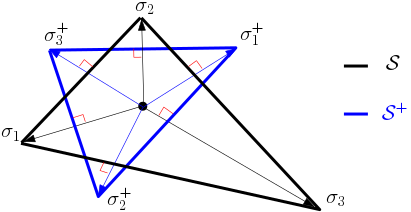
\includegraphics[scale=0.5]{inverse_relations}
	\caption{A simplex of a graph and its inverse. }
	\label{fig:inverse_relations}
\end{figure}

\note{Should hold between every  simplex and its dual. Probably move into prelims section}
\begin{lemma}
\label{lem:faces_orthogonal}
Let $\splx$ and $\splx^+$ be the simplex and inverse simplex of a graph $G=(V,E)$. For any non-empty $U\subset V$,  
the faces $\splx^+_U$ and $\splx_{U^c}$ are orthogonal. In other words, if $\p_1,\p_2\in \splx_U^+$ and $\q_1,\q_2\in \splx_{U^c}$, then $\la \p_1-\p_2,\q_1-\q_2\ra=0$. 
\end{lemma}
\begin{proof}
Let $\p\in \splx^+_U$ and $\q\in \splx_{U^c}$. Letting their barycentric coordinates be $\x_{\p}$ and $\x_{\q}$ respectively, write 
\[\la \p,\q\ra = \x_{\p} (\Sv^+)^\tp \Sv \x_{\q}=\x_{\p}(\I-\one\one^\tp/n) \x_{\q},\]
where we've employed Equation \eqref{eq:sv+sv}. Now, $\x_{\p}(i)=0$ for all $i\in U^c$ and $\x_{\q}(j)=0$ for all $j\in U$. Therefore, $\la \x_{\p},\x_{\q}\ra =0$. Moreover, $\norm{\x_{\p}}_1=\norm{\x_{\q}}_1=1$ and so the above simplifies to $\la \p,\q\ra = -1/n$. Consequently, if $\p_1,\p_2\in \splx_U^+$ and $\q_1,\q_2\in\splx_{U^c}$ we have 
\[\la \p_1-\p_2,\q_1-\q_2\ra = 0,\]
completing the proof. 
\end{proof}

The following lemma presents an alternate characterization of the simplex. 

\begin{lemma}
\label{lem:S_alt_desc}
For a simplex $\splx$ of a graph $G$, 
\begin{equation}
\label{eq:S_alt_desc}
    \splx=\bigg\{\x\in \R^{n-1}:\x^\tp\Sv^++\frac{\one^\tp}{n}\geq \zero^\tp\bigg\}.
\end{equation}
\end{lemma}
\begin{proof}
Put $E=\{\x\in \R^{n-1}:\x^\tp\Sv^++\one^\tp/n\geq \zero^\tp\}$. First we show that $E\subset\splx$. 
Since $\rank(\Sv)=n-1$, it follows that given any $\x\in E$ (indeed, any $\x\in\R^{n-1}$) we can write $\x=\Sv\y$ for some $\y\in\R^n$. Letting $\bar{y}=n^{-1}\sum_i y(i)$ be the mean of the vector $\y$, compute
\begin{align*}
    \x^\tp\Sv^+ &= \y^\tp \Sv^\tp\Sv^+ = \y^\tp(\I-\one\one^\tp/n)=\y^\tp - \bar{y}\one^\tp.
\end{align*}
If $\x\in E$ the above implies that 
\[\y^\tp-\bar{y}\one^\tp + \one^\tp/n\geq \zero^\tp.\]
Moreover, since $\Sv\one=\zero$, we have $\x=\Sv\y=\Sv(\y-\bar{y}\one +\one/n)$. Noticing that 
\[\la \y-\bar{y}\one+\one^\tp/n,\one\ra = n\bar{y}-n\bar{y}+1=1,\]
demonstrates that the vector $\widetilde{\y}=\y-\bar{y}\one+\one^\tp/n$ is a barycentric coordinate for $\x$, and so $\x\in \splx$. 

Conversely, for $\x\in\splx$ let $\y$ be its barycentric coordinate. Then 
\[\x^\tp\Sv^++\one^\tp/n=\y^\tp(\I-\one\one^\tp/n)+\one^\tp/n=\y^\tp - \one^\tp/n+\one^\tp/n=\y^\tp\geq \zero^\tp, \]
hence $\splx\subset E$. This completes the proof. 
\end{proof}

\begin{lemma}
\label{lem:SUsubset}
Let $\splx$ be the simplex of a graph $G=(V,E,w)$, and fix $U\subset V$. For any non-empty $E\subset U^c$,
\begin{equation*}
    \splx_U \subset \bigg\{\x\in\R^{n-1}: \sum_{i\in E}\la \x,\sv_i^+\ra +\frac{|E|}{n}=  0\bigg\},
\end{equation*}
and
\begin{equation*}
    \splx^+_U \subset \bigg\{\x\in\R^{n-1}: \sum_{i\in E}\la \x,\sv_i\ra +\frac{|E|}{n}=  0\bigg\},
\end{equation*}
\end{lemma}
\begin{proof}
Let $\x\in\splx_U$ be arbitrary. For any $i\in U^c$ we have $\la \x,\sv_i^+\ra = -1/n$. Hence, for any $E\subset U^c$
\[\sum_{i\in E}\la \x,\sv_i^+\ra + \frac{|E|}{n} = \sum_{i\in E}\bigg(\la \x,\sv_i^+\ra+\frac{1}{n}\bigg)=\sum_{i\in E}\bigg(\frac{1}{n}-\frac{1}{n}\bigg)=0,\]
implying that $\x$ is in the desired set. 
\end{proof}

Lemma \ref{lem:SUsubset} gives us an alternate way to prove Lemma \ref{lem:S_alt_desc}. For any $i$,  taking $U=N\setminus \{i\}$ and $E=\{i\}$, it implies that $\splx_{\{i\}^c}$ is a subset of the hyperplane 
\[ \H_i\equiv \{\x\in\R^{n-1}:\la \x,\sv_i^+\ra+1/n=0\}.\]
All points in the simplex $\splx$ lie to one side of $\splx_{\{i\}^c}$, i.e., they lie in the halfspace 
\[\H_i^{\geq } \equiv \{\x\in\R^{n-1}:\la \x,\sv_i^+\ra+1/n\geq0\}.\]
(We know it is this halfspace because $\zero\in\splx\cap\H_i^{\geq }$.) The simplex is the interior of the region defined by the intersection of the faces $\splx_{\{i\}^c}$, i.e.,   
\begin{equation}
\label{eq:splx_bigcapH_i}
    \splx=\bigcap_i \H_i^{\geq }.
\end{equation}
Moreover, $\x\in \bigcap_i\H_i^{\geq }$ iff $\la \x,\sv_i^+\ra +1/n\geq 0$ for all $i$, i.e., $(\la \x,\sv_1^+\ra,\dots,\la \x,\sv_n^+\ra) + \one/n\geq \zero$, meaning $\x$ satisfies \eqref{eq:S_alt_desc}.  We emphasize that a very similar discussion applies to $\splx^+$, in which case one has 
\begin{equation}
\label{eq:splx^+_bigcapH_i}
\splx=\bigcap_i (\H_i^+)^{\geq },
\end{equation}
for $(\H_i^+)^{\geq } \equiv \{\x\in\R^{n-1}:\la \x,\sv_i\ra + 1/n\geq 0\}$. 






\paragraph{Global Connectivity}
Given $U\subset V(G)$ then \emph{cut-set} of $U$ is 
\[\delta U \equiv (U\times U^c)\cap E(G)= \{(i,j)\in E(G): i\in U, j\in U^c\}.\]
Noting that $|\chi_U(i)-\chi_U(j)|=\chi_{(i,j)\in \delta U}$, we see that
\begin{align*}
    w(\delta U) = \sum_{i,j\in E} w(i,j)|\chi_U(i)-\chi_U(j)| = \sum_{i,j\in E} w(i,j)(\chi_U(i)-\chi_U(j))^2 = \Lf(\chi_U). 
\end{align*}
Moreover, $\norm{c(\splx_U)}^2_2 = \la |U|^{-1} \Sigma\chi_U,|U|^{-1} \Sigma\chi_U\ra = |U|^{-2} \Lf(\chi_U)$ and so 
\begin{equation}
\label{eq:c(S_U)}
    \norm{c(\splx_U)}_2^2 = \frac{w(\delta U)}{|U|^2}.
\end{equation}
Via the same process we can also obtain an equivalent expression for the centroid of the inverse simplex: 
\begin{equation}
\label{eq:c(S+_U)}
    \norm{c(\splx^+_U)}_2^2 = \frac{w(\delta^+ U)}{|U|^2},
\end{equation}
where we define $w(\delta^+U) \equiv  \la \Sv^+\chi_U,\Sv^+\chi_U\ra=\la \chi_U,\L^+\chi_U\ra$. 




\subsubsection{Centroid and Altitudes}
Recall that the altitude between $\splx[U]$ and $\splx[U^c]$ of a simplex $\splx$ is the unique vector $\p-\q$ where  $\p\in \splx_{U^c}$ and $\q\in\splx_{U}$ which lies in the orthogonal complement of both $\splx_U$ and $\splx_{U^c}$. 

\begin{lemma}
\label{lem:complimentary_centroids}
Let $U\subset V$ be non-empty. Then the vectors $c(\splx_U)$ and $c(\splx_{U^c})$ are antiparallel. In particular, $(n-|U|)c_{U^c} = |U|c_{U}$ and 
\[\frac{c_U}{\norm{c_U}_2}=-\frac{c_{U^c}}{\norm{c_{U^c}}_2}.\]
\end{lemma}
\begin{proof}
This is a straightforward computation: Observing that $\chi_U=n-\chi_{U^c}$ we have  
\[c_U = |U|^{-1}\Sv\chi_U = |U|^{-1}\Sv(\one-\chi_{U^c})=-|U|^{-1}\Sv\chi_{U^c}=-|U|^{-1}\frac{|U^c|}{|U^c|}\Sv\chi_{U^c}=\frac{n-|U|}{|U|}c_{U^c},\]
where we've used that $\Sv\one=\zero$. This proves the first result; the second follows from normalizing the two vectors.
\end{proof}

\begin{lemma}
\label{lem:alt_and_centroid}
For a simplex $\splx$ of a graph $G=(V,E)$ and any $U\subset V$, $U\neq\emptyset$, 
\begin{equation*}
    \frac{\alt(\splx_U)}{\norm{\alt(\splx_{U})}_2}=\frac{c^+(\splx_{U^c})}{\norm{c^+(\splx_{U^c})}_2}=-\frac{c^+(\splx_{U})}{\norm{c^+(\splx_{U})}_2},
\end{equation*}
and 
\begin{equation*}
    \frac{\alt^+(\splx_U)}{\norm{\alt^+(\splx_{U})}_2}=\frac{c(\splx_{U^c})}{\norm{c(\splx_{U^c})}_2}=-\frac{c(\splx_{U})}{\norm{c(\splx_{U})}_2}.
\end{equation*}
\end{lemma}
\begin{proof}
We prove the first set of  equalities only; the second is obtained similarly. 
Put $\alt_U=\alt(\splx_U)$ and $c_U=c(\splx_U)$. By definition, $\alt_U$ is orthogonal to both $\splx_U$ and $\splx_{U^c}$. \note{need the following claim: Any vector perpendicular to $\splx_U$ can be written as $\Sv^+x_{U^c}$. Why the hell is this true? $\splx^+x_{U^c}$ represents the simplex $\splx^+_{U^c}$ which we know is perpendicular to $\splx_U$. However, does it follow it is the \emph{only} thing perpendicular to $\splx_U$?? } Since $\alt_U$ begins at $\splx_U$ and ends at $\splx_{U^c}$ it follows that 
\begin{equation*}
    \frac{\alt_U}{\norm{\alt_U}_2}=-\frac{\Sv^+f_{U^c}}{\norm{\Sv^+f_{U^c}}_2}=\frac{\Sv^+f_{U}}{\norm{\Sv^+f_{U}}_2}.
\end{equation*}
By Lemma \ref{lem:complimentary_centroids}, taking $f_{U^c}=\chi_{U^c}/|U^c|$ and $f_U=\chi_U/|U|$ yields a solution to the above equation. We claim there are no other solutions, up to scaling. Indeed, let $g_{U^c}$ and $g_U$ satisfy the above, and normalize them so that $\norm{\Sv^+g_{U^c}}_2=\norm{\Sv^+g_U}_2=1$. Then we have $\Sv^+(g_U+g_{U^c})=0$ and so $g_U+g_{U^c}=k\one$ since $\ker(\Sv^+)=\spn(\{\one\})$. Hence $g_U$ and $g_{U^c}$ are scaled versions of $f_U$ and $f_{U^c}$.  
\end{proof}

\begin{lemma}
\label{lem:||alt||}
For any non-empty $U\subset V$, $\norm{a^+_U}_2^2=1/w(\delta U)$ and $\norm{a_U}_2^2 = 1/w(\delta^+ U)$.  
\end{lemma}
\begin{proof}
By definition of the altitude there exists barycentric coordinates $\x_U$ and $\x_{U^c}$ such that $a^+U = \Sv^+(\x_U-\x_{U^c})$. Combining this representation of $a^+_U$ with that given by Lemma \ref{lem:alt_and_centroid}, write 
\begin{align*}
    \norm{a^+_U}_2 = \frac{\la a^+_U,a^+_U\ra }{\norm{a^+_U}_2} = \frac{\la \Sv^+(\x_{U^c}-\x_{U}), c_{U^c}\ra }{\norm{c_{U^c}}_2} = \frac{\la \Sv^+(\x_{U^c}-\x_{U}), \Sv\bchi_{U^c}\ra }{\sqrt{w(\delta U^c)}},
\end{align*}
where the final equality comes from using the definition of the centroid in the numerator, and Equation \ref{eq:c(S_U)} in the denominator. Recalling the relation between $\Sv$ and $\Sv^+$ given by Equation \ref{eq:sv+sv} and that $\x_U$ and $\x_{U^c}$ are barycentric coordinates, we can rewrite the above as 
\[\frac{(\x_{U^c}-\x_{U})^\tp(\I-\one\one^\tp/n)\bchi_{U^c}}{\sqrt{w(\delta U^c)}}=\frac{1}{\sqrt{w(\delta U^c)}}. \]
Squaring both sides while noting that $\delta U = \delta U^c$ completes the proof of the first equality. For the second, we proceed in precisely the same manner to obtain $\norm{a_U}_2^2 = 1/w(\delta^+ U^c)$. However, it's not immediately obvious that $w(\delta^+U^c)=w(\delta^+U)$. To see this, first recall that $\Sv^+\one = \Eval^{-1/2}\Eig^\tp\one = \zero$, and so 
\begin{align*}
w(\delta^+ U^c) &= \la \Sv^+\bchi_{U^c},\Sv^+\bchi_{U^c}\ra  \\
&= \la \Sv^+(\one - \bchi_{U}),\Sv^+(\one - \bchi_{U})\ra  \\
&= \la \Sv^+\bchi_{U},\Sv^+\bchi_{U}\ra = w(\delta^+ U).
\qedhere
\end{align*}
\end{proof}


\begin{lemma}
\label{lem:svi^+ai_parallel}
The vectors $\sv_i^+$ and $\alt(\splx_i)$ are antiparallel. 
\end{lemma}
\begin{proof}
First, notice that $\sv_i^+=\bchi_i \Sv^+=\cent(\splx^+_{\{i\}})$ and so \begin{equation*}
    \norm{\sv_i^+}_2 = \norm{\cent(\splx^+_{\{i\}})}_2 = \norm{ w(\delta^+ \{i\})}_2 = \frac{1}{\norm{\alt_i}}_2,
\end{equation*}
where the penultimate and final inequalities follow from Equation \eqref{eq:c(S+_U)} and Lemma \ref{lem:||alt||}, respectively. Let $\x=\x_{\{i\}^c}$ be the barycentric coordinate of the face $\S_{\{i\}^c}$ such that $\alt_i = \Sv(\x-\bchi_i)$. Then, 
\begin{align*}
    \bigg\la \frac{\sv_i^+}{\norm{\sv_i}_2},\frac{\alt_i}{\norm{\alt_i}_2}\bigg \ra 
    &= \frac{1}{\norm{\sv^+_i}_2\norm{\alt_i}_2} \bigg( \la \sv_i^+,\Sv\x\ra - \la \sv_i^+,\Sv\bchi_i\ra \bigg) \\
    &= \bchi_i^\tp (\Sv^+)^\tp \Sv \x - \bchi_i^\tp (\Sv^+)^\tp \Sv\bchi \\
    &= \bchi_i^\tp (\I-\J/n) \x - \bchi_i^\tp(\I-\J/n) \bchi_i \\
    &= - \frac{\bchi_i^\tp \one\one^\tp \x }{n} - 1 + \frac{\bchi_i^\tp \one\one^\tp \bchi_i}{n}=-1,
\end{align*}
since $\one^\tp \x=\one^\tp \bchi_i=1$. 
\end{proof}

\begin{lemma}
\label{lem:alt}
For any non-empty $U\subset V$, 
\[\alt_U=\frac{n-|U|}{w(\delta^+ U)}\cent^+_{U^c},\quad \text{and}\quad \alt^+_U = \frac{n-|U|}{w(\delta U)} \cent_{U^c}.\]
\end{lemma}
\begin{proof}
This is a consequence of identities \eqref{eq:c(S_U)} and \eqref{eq:c(S+_U)} and Lemmas \ref{lem:alt_and_centroid} and \ref{lem:||alt||}. Applying the latter and then the former, observe that 
\[\alt_U = \frac{\norm{\alt_U}_2}{\norm{\cent^+_{U^c}}_2}\cent^+_{U^c} =
\bigg(\frac{1}{\sqrt{w(\delta^+ U^c)}} \bigg/\frac{\sqrt{w(\delta^+U)}}{|U^c|} \bigg)\cent^+_{U^c} = \frac{n-|U|}{w(\delta^+U)}c^+_{U^c},\]
where we've once against used that $w(\delta^+ U^c )=w(\delta^+ U)$. A similar computation holds for $\alt_U^+$.  
\end{proof}


\begin{lemma}
Let $G=(V,E,w)$ be a weighted, undirected graph. Then 
\begin{equation*}
    \la c(\splx_{U_1}),c(\splx_{U_2})\ra = - \frac{w(\delta U_1\cap \delta U_2)}{|U_1||U_2|},\quad\text{and}\quad \la \alt^+_{U_1},\alt^+_{U_2}\ra = -\frac{w(\delta U_1^c\cap \delta U_2^c)}{w(\delta U_1)w(\delta U_2)}.
\end{equation*}
\end{lemma}
\begin{proof}
For $i,j\in V$, observe that $\chi_{U_1}^\tp \L_e\chi_{U_2}=-w(i,j)$. Therefore, 
\begin{align*}
    \la c_{U_1},c_{U_2}\ra &= \la |U_1|^{-1}\Sv\chi_{U_1},|U_2|^{-1}\Sv\chi_{U_2}\ra = |U_1|^{-1}|U_2|^{-1} \chi_{U_1}^\tp \L_G\chi_{U_2} \\
    &= |U_1|^{-1}|U_2|^{-1}\sum_{i\sim j} \chi_{U_1}^\tp \L_{(i,j)}\chi_{U_2} = |U_1|^{-1}|U_2|^{-1}\sum_{(i,j)\in \delta U_1\cap \delta U_2} -w(i,j),
\end{align*}
which proves the first equality. The second is shown similarly by employing Lemma \ref{lem:alt} and the previous identity:
\begin{align*}
    \la \alt^+_{U_1},\alt^+_{U_2}\ra &= \frac{|U_1^c||U_2^c|}{w(\delta U_1) w(\delta U_2)}\la c_{U_1^c},c_{U_2^c}\ra
    =-\frac{w(\delta U_1^c\cap \delta U_2^c)}{w(\delta U_1)w(\delta U_2)}.\qedhere
\end{align*}

\end{proof}

\section{Properties of \texorpdfstring{$\splxn_G$}{the normalized Simplex} and \texorpdfstring{$\splxn_G^+$}{and its inverse}}
\label{sec:Sn_G}

Here we study the normalized simplex $\splxn_G$ of the graph $G$, a somewhat less accessible object than its unnormalized counterpart.  The normalized simplex is, roughly speaking, distorted by the weights of the vertices. Consequently, many of the relationships between $\splx_G$ and $\splx_G^+$ are lost between $\splxn_G$ and $\splxn_G^+$. The first issue is that, in general, $\splxn_G$ and its inverse are not centred at the origin. Indeed, recall that the zero eigenvector $\vpn_n$ of $\Ln_G$ sits in the space $\spn(\W^{1/2}_G\one)$, which is distinct from $\spn(\one)$ unless $\W^{1/2}_G=d\I$ for some $d$, in which case $G$ is regular.
If $G$ is not regular, we thus have that $\vp_i \in \spn(\W^{1/2}_G\one)\subset \spn(\one)^\perp$ for all $i<n$ implying that $\la \vp_i,\one\ra \neq 0$. In this case then,  
 \[\cent(\splxn_G) = \frac{1}{n} \Evaln^{1/2}\Eign^\tp \one = \frac{1}{n} \begin{pmatrix}
 \sqrt{\lambda_1}\la \vp_1,\one\ra \\
 \vdots \\
\sqrt{ \lambda_{n-1}}\la \vp_{n-1},\one \ra
 \end{pmatrix}\neq \zero.\]
The above argument proves the following.

\begin{lemma}
	\label{lem:centroid_normalized}
	The centroid of $\splxn_G$ coincides with the origin of $\R^{n-1}$ iff $G$ is regular. 
\end{lemma}

Given this, one might wonder whether the origin is even a point in the simplex $\splxn$. It is easily seen that it is, however. Consider the barycentric coordinate $\u = \sqrt{\w}/\norm{\sqrt{\w}}_1$, where $\sqrt{\w}=(w(1)^{1/2}, \dots, w(n)^{1/2})$. Since all eigenvectors $\vpn_i$, $i<n$ are orthogonal to $\vp_n \in\spn(\w^{1/2})$ it follows that $\zero = \Svn\u\in\splxn$. 

The next set of properties which don't hold between $\splxn$ and $\splxn^+$ are the orthogonality relationships present between a simplex and its dual. That is, in general $\splxn^+_G$ is the not the dual of $\splxn_G$. 

\begin{lemma}
	\label{lem:inverse_not_dual}
	The inverse simplex $\splxn_G^+$ is the dual of $\splxn_G$ iff $G$ is regular. 
\end{lemma}
\begin{proof}
	For any $i,j,k\in\N$ write 
	\begin{equation}
	\label{eq:lem_inverse_not_dual}
	\la \svn_i^+,\svn_j-\svn_k\ra = \delta_{ij} - \delta_{ik} + \frac{\sqrt{w(i)w(k)}}{n} - \frac{\sqrt{w(i)w(j)}}{n}.
	\end{equation}
	First suppose that $G$ is $k$-regular. Then for $i\neq k$, Equation \eqref{eq:lem_inverse_not_dual} becomes $\la \svn_i^+,\svn_j-\svn_k\ra = \delta{ij}$. Since $k$ was arbitrary, we see that $\{\svn_i^+\}$ is the sister pair of $\{\svn_j-\svn_k\}$. Conversely, suppose $G$ is not regular and let $i,k$ obey $0\neq w(i)\neq w(k)$. Taking $i=j\neq k$ in \eqref{eq:lem_inverse_not_dual} we see 
	\[\la \svn_i^+,\svn_i-\svn_k\ra = 1 - \frac{\sqrt{w(i)}}{n}(\sqrt{w(k)}-\sqrt{w(i)})\neq 1,\]
	so $\{\svn_i^+\}$ is not the sister set of $\{\svn_j-\svn_k\}$, completing the argument. 
\end{proof}


Recall from Section \ref{sec:background_spectral} that a subset of vertices is degree homogenous if each vertex in the set has the same weight. 

\begin{lemma}
	\label{lem:Sn_perp_homogenous}
	Let $U_1,U_2\subset V(G)$ be two non-empty, degree homogenous subsets such that $U_1\cap U_2=\emptyset$. Then the faces $\splxn^+[U_1]$ and $\splxn[U_2]$ are perpendicular. 
\end{lemma}
\begin{proof}
	Suppose $w(i)=w_1$ for all $i\in U_1$ and $w(i)=w_2$ for all $i\in U_2$. Let $\x_{U_1}$ be the barycentric coordinate of any point in $\splxn^+[U_1]$ and $\x_{U_2}$ that of any point in $\splxn[U_2]$. 
	\begin{align*}
	\la \Svn^+\x_{U_1},\Svn\x_{U_2}\ra &= \x_{U_1}^\tp \bigg(\I-\frac{\sqrt{\w}\sqrt{\w}^\tp}{\vol(G)}\bigg) \x_{U_2}\\
	&= \x_{U_1}^\tp\x_{U_2} - \frac{1}{\vol(G)}\sum_{i\in U_1}\x_{U_1}(i)\sqrt{w(i)}\sum_{j\in U_2}\x_{U_2}(j) \sqrt{w(j)} \\
	&= -\frac{1}{\vol(G)}\sqrt{w_1w_2}\sum_{i\in U_1}\x_{U_1}(i) \sum_{j\in U_2}\x_{U_2}(j) = -\frac{\sqrt{w_1w_2}}{\vol(G)},
	\end{align*} 
	where the second equality is due to fact that $U_1\cap U_2=\emptyset$. This demonstrates that $\la \Svn^+\x_{U_1},\p-\q\ra=0$ for any $\p,\q\in\splxn[U_2]$, completing the proof. 
\end{proof}

\begin{lemma}
	\label{lem:Sn_not_homogeneous}
	Suppose  $U_1\subset V(G)$ is not degree homogeneous. Then for all $U_2\subset V(G)$ then faces $\splxn[U_1]$ (resp., $\splxn^+[U_1]$) and $\splxn^+[U_2]$ (resp., $\splxn[U_2]$) are not perpendicular. 
\end{lemma}
\begin{proof}
	We show that $\splxn[U_1]$ and $\splxn^+[U_2]$ are not orthogonal; the other case is nearly identical. Let $i,j\in U_1$ be such that $w(i)\neq w(j)$ and consider the points $\p=\Svn\bchi_i,\q=\Svn\bchi_j\in\splxn[U_1]$. For any $\Svn^+\x\in\splxn^+[U_2]$, performing the usual arithmetic yields
	\begin{align*}
	\la \Svn^+\x,\p-\q\ra &= \frac{1}{\vol(G)} \sum_{k\in U_2}\sqrt{w(k)}x(k)(\sqrt{w(j)}-\sqrt{w(j)}) \neq 0.\qedhere
	\end{align*}
\end{proof}

\begin{corollary}
	\label{cor:Sn_orthog_iff_regular}
	The vertex $\svn_i^+$ (resp., $\svn_i$) is orthogonal to $\splxn_\ic$ (resp., $\splxn^+_\ic$) iff $G[\ic]=G[V\setminus\{i\}]$ is regular. 
\end{corollary}
\begin{proof}
	If $G[\ic]$ is regular then $\ic$ is weight homogenous. By Lemma~\ref{lem:Sn_perp_homogenous} $\splxn[\{i\}]=\svn_i$ (resp., $\splxn^+[\{i\}]=\svn_i^+$) is orthogonal to $\splxn[\ic]$ (resp., $\splxn^+[\ic]$). (Note that the singleton $\{i\}$ is clearly degree homogeneous.) Conversely, if $G[\ic]$ is not regular then by Lemma~\ref{lem:Sn_not_homogeneous} $\svn_i$ (resp., $\svn_i^+$) is not orthogonal to $\splxn[\ic]$ (resp., $\splxn^+[\ic]$).
\end{proof}

\paragraph{Centroids and Altitudes.}
For the normalized Laplacian we have
\begin{align}
\Lnf(\bchi_U)&=\sum_{i\sim j}w(i,j) \bigg(\frac{\bchi_U(i)}{\sqrt{w(i)}}-\frac{\bchi_U(j)}{\sqrt{w(j)}}\bigg)^2 \notag \\
&= \sum_{i\in U,j\in U^c}w(i,j)\bigg(\frac{\bchi_U(i)}{\sqrt{w(i)}}-\frac{\bchi_U(j)}{\sqrt{w(j)}}\bigg)^2 \notag \\
&= \sum_{i\in U,j\in U^c}w(i,j)\frac{\bchi_U(i)}{w(i)} \notag \\
&= \sum_{i\in U}\frac{1}{w(i)} \sum_{j\in \delta(i)\cap U^c}w(i,j) \notag \\
&= \sum_{i\in U}\frac{w_{G[i+U^c]}(i)}{w(i)}, \label{eq:Lnf(chiU)}
\end{align}
where we've used the shorthand $i+U^c = \{i\}\cup U^c$ and we recall that $G[I]$ is the graph restricted to the vertices in $I$. In words then, the quantity 
\[\gamma(i,B)\equiv \frac{w_{G[i+U^c]}(i)}{w(i)},\]
is the \emph{fractional weight of $i$ in $B$}. 
Further defining $\gamma(A,B)$ as the \emph{total fractional weight from $A$ to $B$}:
\[\gamma(A,B) \equiv \sum_{i\in A}\gamma(i,B), \]
we have 
\[\Lnf(\bchi_U) = \gamma(U,U^c),\]
and so
\begin{equation}
\label{eq:c(SnU)}
\norm{c(\splxn_U)}_2^2 = \frac{1}{|U|^2}\la \Svn\chi_U,\Svn\chi_U\ra = \frac{1}{|U|^2}\Lnf(\chi_U) = \frac{1}{|U|} \gamma(U,U^c).
\end{equation}


That is, the length of the centroid $c(\splxn_U)$ captures the total fraction of weight between $U$ and $U^c$. 
 
 
The lemma equivalent to \ref{lem:SUsubset} for the normalized simplex is as follows. 

\begin{lemma}
	\label{lem:SUn_subset}
	Let $U\subset V$ be non-empty and $F\subset U^c$. Setting 
	\[\beta_i^S = \sqrt{w(i)} \frac{\max_{j\in S} \sqrt{w(j)}}{\vol(G)},\]
	for any set $S$, we have 
	\begin{equation*}
	\splxn_U \subset \Hn_{F}^\geq \equiv \bigg\{\x\in\R^{n-1}: \sum_{i\in F} (\la \x,\svn_i^+\ra + \beta_i^{F^c})\ge 0\bigg\}.
	\end{equation*}
	Similarly, 
	\begin{equation*}
	\splxn^+_U \subset (\Hn^+_{F})^\geq \equiv \bigg\{\x\in\R^{n-1}: \sum_{i\in F} (\la \x,\svn_i\ra + \beta_i^{F^c})\ge 0\bigg\}.
	\end{equation*}
\end{lemma} 
\begin{proof}
	Let $\x=\Svn\y\in \splxn_U$, where $\y$  is a barycentric coordinate with $\y(U^c)=\zero$. For $i\in U^c$, 
	\begin{align*}
	\la \Svn\y,\svn_i^+ \ra &= \y^\tp \Svn^\tp \Svn^+ \bchi_i = \y^\tp \bigg(\I-\frac{\sqrt{\w}\sqrt{\w}^\tp}{\vol(G)}\bigg)\bchi_i = - \frac{1}{\vol(G)} \left(\sum_{j\in U}y(j) \sqrt{w(j)}\right) \sqrt{w(i)}.
	\end{align*}
	Since $\norm{\y}_1=1$, and $F^c\supset U$ (since $F\subset U^c$) it follows that 
	\[\sum_{j\in U}y(i) \sqrt{w(j)} \leq \max_{j\in U} \sqrt{w(j)} \leq \max_{j\in F^c}\sqrt{w(j)},\]
	hence 
	\[\la \Svn\y,\svn_i^+\ra \geq -\frac{\sqrt{w(i)}}{\vol(G)} \max_{j\in F^c}\sqrt{\w(j)} = -\beta_i^{F^c}.\]  
	Consequently, $\sum_{i\in F} (\la \x,\svn_i^+\ra + \beta_i^{F_c}) \geq \sum_{i\in F^c}(-\beta_i^{F^c} +\beta_i^{F^c})=0$, so indeed $\x\in \Hn_F$. The proof for the $\splxn^+_G$ and $\Hn_F^+$ is almost identical. 
\end{proof}

We might expect that Lemma \ref{lem:SUn_subset} yields a hyperplane representation of the normalized simplex, as did \ref{lem:SUsubset} for the combinatorial simplex. Unfortunately however, the issue is once again complicated by the vertex weights and the relation between $\Svn^+$ and $\Svn$. Let us illustrate the problem by focusing on $\splxn$. 

As opposed to Section \ref{sec:S_G}, $\splxn_\ic $ is not contained in the hyperplane $\Hn_i = \{\x: \la \x,\svn_i^+\ra + \beta_i=0\}$, where we take $\beta_i = \beta_i^{\{i\}^c} = \sqrt{w(i)}\max_{j\neq i}\sqrt{w(j)} / \vol(G)$. To see this, take any $k\notin \argmax_{j\neq i} \sqrt{w(j)}$ (such a $k$ exists iff the graph is not regular) and note that while $\sv_k\in\splxn_U$ it is not in $\Hn_i$: 
\[\la \sv_k,\sv_i^+\ra = \bchi_k\Svn^\tp\Svn^+\bchi_i = -\frac{\sqrt{w(k)w(i)}}{\vol(G)}\neq \beta_i,\]
by assumption. The other way to see this is to note that $\svn_i^+$ is not perpendicular to $\splx_\ic$ in general by Corollary \ref{cor:Sn_orthog_iff_regular}. 



Noting that 
\begin{equation*}
\cent(\splxn) = \frac{1}{n}\bigg(\sum_{\ell=1}^n \svn_\ell(1),\dots,\sum_{\ell=1}^n \svn_\ell(n)\bigg)^\tp,
\end{equation*}
we see that the vertices of $\splxn_0$ have coordinates
\begin{equation*}
\svn_i(j) - \cent(\splxn)(j) = \vpn_j(i)\lambdan_j^{1/2} - \frac{1}{n}\sum_{\ell=1}^n \vpn_j(\ell)\lambdan_j^{1/2} = \lambdan_j^{1/2} \bigg(\vpn_j(i) - \frac{1}{n}\la \vpn_j,\one\ra \bigg).
\end{equation*}
Likewise, the vertices of $\splx_0^+$ have coordinates 
\begin{equation*}
\svn_i^+(j) = \evaln_j^{-1/2}\bigg(\vpn_j(i) - \frac{1}{n}\la \vpn_j,\one\ra\bigg).
\end{equation*}


In light of Lemma \ref{lem:SUsubset}, one might imagine that if given a simplex in \hdesc, say $\ssplx=\bigcap_i \{\x:\la \z_i,\x\ra \geq b_i\}$ then the vectors $\z_i$ are parallel to the dual vertices of $\ssplx$. Lemma~\ref{lem:SUn_subset}, however, disconfirms this hypothesis. As is illustrated by some ugly arithmetic in Section~\ref{sec:Sn_G}, the dual vertices of $\splxn_G$ are not $\{\svn_i^+\}$, but $\splxn_G = \bigcap_i \{\x:\la \x,\svn_i^+\ra \geq \beta_i/n\}$ by Equation \eqref{eq:Sn_altdesc}. It turns out the key difference is that $\splx_G$ is centred whereas $\splxn_G$ is not. 

\begin{lemma}
	\label{lem:hdesc_dual}
	Let $\ssplx\subset\R^{n-1}$ be a centred simplex with $\ssplx=\bigcap_{i=1}^n  \{\x\in\R^{n-1}: \la \x,\z_i\ra \geq  \alpha_i\}$. Then $\{-\z_i/(\alpha_i n)\}$ are the vertices of $\ssplx^D$. 
\end{lemma}
\begin{proof}
	As usual, let $\{\sv_i\}$ be the vertices of $\ssplx$. Put $\bgamma_i = -\z_i/(\alpha_i n)$. We need to show that $\{\bgamma_i\}_{i=1}^{n-1}$ is the sister basis to $\{\sv_i-\sv_n\}_{i=1}^{n-1}$. Let $H_i$ be the boundary of the halfspace $\{\x:\la \x,\z_i\ra \geq \alpha_i\}$, so $H_i = \{\x:\la \x,\z_i\ra = \alpha_i\}$. Enumerate the vertices $\{\sv_i\}$ such that $\splx_\ic \subset H_i$. Fix $i\in[n-1]$. We claim that 
	\[\sv_i \in \bigcap_{j\neq i}H_i.\]
	Indeed, $\splx_\jc$ is the $n-1$ dimensional simplex with vertices $\{\sv_\ell\}_{\ell\neq j}$. Hence $\sv_i\in \splx_\jc$ for all $j\neq i$ and thus also lies in $\cap_{j \neq i}H_j$. Therefore, $\la \sv_i,\z_j\ra = \alpha_j$ for all $j\neq i$, from which it follows  that $\la \bgamma_j,\sv_i-\sv_n\ra = -\la \z_j,\sv_i\ra/(\alpha_j n) + \la \z_j,\sv_n\ra / (\alpha_j n )=1/n - 1/n =0$.  
	It remains to show that $\la \bgamma_i,\sv_i-\sv_n\ra=1$ for all $i\neq n$. Since $\ssplx$ is centred by assumption, we have $\sv_i = -\sum_{j\neq i} \sv_j$. Consequently, 
	\begin{align*}
	\la \bgamma_i,\sv_i-\sv_n\ra &= -\sum_{j\neq i}\la \bgamma_i,\sv_j\ra - \la \bgamma_i,\sv_n \ra = \frac{1}{n}(n-1) + \frac{1}{n} = 1,
	\end{align*}
	as was to be shown.  
\end{proof}

\begin{lemma}
	\label{lem:hdesc_centred}
	Let $\ssplx=\cap_i \{\x:\la \x,\z_i\ra \geq \alpha_i\}$ be a simplex. Its centred version, $\ssplx_0$, can be written as $\cap_i \{\x:\la \x,\z_i\ra \geq \alpha_i - \la \cent(\ssplx),\z_i\ra\}$. 
\end{lemma}
\begin{proof}
	As usual, take $\H_i = \{\x:\la \x,\z_i\ra = \alpha_i\}$ to be the hyperplanes bounding the simplex. The hyperplanes bounding the centred simplex, are parallel to the hyperplanes $\H_i$ and can thus be written as 
	\[\H_{i0} = \{\x:\la \x,\z_i\ra = \beta_i\},\]
	for some $\beta_i$. Moreover, just as $\sv_j\in\H_i$ for $j\neq i$, we have $\sv_j-\cent(\ssplx)\in \H_{i0}$, since $\{\sv_j-\cent(\ssplx)\}$ are the vertices of $\ssplx_0$. As such, $\la \sv_j-\cent(\ssplx),\z_i\ra=\beta_i$, and 
	\[\la \sv_j-\cent(\ssplx),\z_i\ra = \la \sv_j,\z_i\ra - \la\cent(\ssplx),\z_i\ra = \alpha_i - \la\cent(\ssplx),\z_i\ra,\]
	whence $\beta_i = \alpha_i - \la\cent(\ssplx),\z_i\ra$. It then follows that 
	\[\ssplx_0=\bigcap_i \H_{i0}^{\geq },\]
	where $\H_{i0}^\geq = \{\x:\la \x,\z_i\ra \geq  \alpha_i - \la \cent(\ssplx),
	\z_i\ra\}$. 
\end{proof}

\begin{corollary}
	\label{cor:dual_Sn}
	The dual simplex to $\splxn_G^+$ has vertices 
	\begin{equation*}
	\bigg\{\frac{\svn_i^+}{\beta_i + n\la \cent(\ssplx),\svn_i^+\ra}\bigg\},
	\end{equation*}
	where 
	\[\beta_i = \bigg(w(i)\sum_{j\neq i}w(j)\bigg)^{1/2}.\]
\end{corollary}
\begin{proof}
	Lemma \ref{lem:SUn_subset} and Equation \eqref{eq:Sn_altdesc} tells us that $\splxn = \bigcap_i \H_i^\geq $ where  $\H_i = \{\x:\la \x,\svn^+_i\ra \geq -\beta_i/n\}$. Lemma \ref{lem:hdesc_centred} then implies that 
	\begin{equation*}
	\splxn_0 = \bigcap_i \bigg\{\x:\la \x,\svn_i^+\ra \geq -\frac{\beta_i}{n} - \la \cent(\ssplx),\svn_i^+\ra\bigg\}.
	\end{equation*}
	Put $\kappa_i = -\beta_i/n - \la \cent(\ssplx),\svn_i^+\ra$. 
	Lemma \ref{lem:hdesc_dual} then dictates that the dual vertices of $\splx_0^D$ obey 
	\begin{equation*}
	\bigg\{\frac{\svn_i^+}{-n\cdot \kappa_i}\bigg\} = 	\bigg\{\frac{\svn_i^+}{\beta_i + n\la \cent(\ssplx),\svn_i^+\ra}\bigg\}.
	\end{equation*}
	Finally, since a centred simplex and its uncentred counterpart share the same dual simplex by Observation \ref{obs:dual_centred}, the result follows. 
\end{proof}










\section{Construction via Extended Menger and Gramian}
In this section we derive matrix equations which relate the geometry of hyperacute simplices and their duals. The equations appeal to the relationship between hyperacute simplices and graphs by using well known results from the literature on electrical networks and effective resistance. The goal of this section is to demonstrate to the reader the utility of the graph-simplex correspondence in generating statements about hyperacute simplices, by hijacking our knowledge of graph theory. 

Let a centred, hyperacute simplex $\splx^+$ be given. By Theorem \ref{thm:graph-simplex} it is the inverse simplex of a graph $G$, whose corresponding simplex $\splx = \splx_G$ is dual to $\splx^+$.
Therefore, $\L_G=\Sv^\tp\Sv$ and $\L_G^+=(\Sv^+)^\tp\Sv$ and the vertices $\sv_i^+$ of $\splx^+$ can be written as $\sv_i^+=(\vp_1(i)\lambda_1^{1/2},\dots,\vp_{n-1}(i)\lambda_{n-1}^{1/2})^\tp$. Hence, 

\begin{align*}
\norm{\sv_i^+-\sv_j^+}_2^2 = (\bchi_i-\bchi_j)^\tp (\Sv^+)^\tp\Sv^+ (\bchi_i-\bchi_j) = \effr(i,j).
\end{align*}

That is, the distance between the vertices of $\splx^+$ encodes the effective resistance between nodes $i$ and $j$ in $G$. Let $\D^+$ be the distance matrix of $\splx^+$ (thus the effective resistance matrix $\Reff_G$ of $G$). 


\note{Detour into electrical networks, not sure where this goes exactly.} Observe that starting with the equation $\Reff=\one\diag(\L_G^+(i,i))^\tp + \diag(\L_G^+(i,i))\one^\tp - 2\L_G^+$, \note{should explain where this equation comes from} it follows that $\x^\tp \Reff\x = -2\x^\tp \L_G^+\x$ for any $\x\in\spn(\one)^\perp$. Therefore, 
\begin{align*}
\L_G^+(i,j)&=\bchi_i^\tp \L_G^+\bchi_j \\
&= \bigg(\bchi_i-\frac{1}{n}\one\bigg)^\tp \L_G^+\bigg(\bchi_j-\frac{1}{n}\one\bigg) \\
&= -\frac{1}{2}\bigg(\bchi_i-\frac{1}{n}\one\bigg)^\tp \Reff_G\bigg(\bchi_j-\frac{1}{n}\one\bigg) \\
&= \frac{1}{2n}\bigg(\sum_{k\in[n]}\effr(i,k)+\effr(j,k)\bigg) - \frac{1}{2}\effr(i,j) -\frac{R_G}{n^2},
\end{align*}
where $R_G$ is the total effective resistance of the graph. 
For $i=j$, this becomes 
\begin{align*}
\L_G^+(i,i) = \frac{1}{n} \sum_{k\in[n]}\effr(i,k) - \frac{R_G}{n^2}.
\end{align*}

Let $\overline{d}$ be the average squared distance between all the vertices of $\splx^+$, that is
\[\overline{d} \equiv  \frac{1}{n^2}\sum_{i\leq j} \norm{\sv_i^+-\sv_j^+}_2^2.\]
Let $\xi(i)$ give the average squared distance of vertex $i$ from other vertices minus the total average distance, 
\[\xi(i) \equiv \frac{1}{n}\sum_{j} \norm{\sv_i^+-\sv_j^+}_2^2 - \overline{d},\]
and put $\bxi=(\xi(1),\dots,\xi(n))$. 
Then we have the following result. 

\begin{lemma}
	Let $\splx\subset\R^{n-1}$ be a centred hyperacute simplex with  squared distance matrix $\D$, and average squared distance vector $\bxi$. Denote by $\BGamma$ the vertex matrix of the dual simplex to $\splx$. Then, 
	\begin{equation}
	\label{eq:simplex_block_matrix}
	-\frac{1}{2} \begin{pmatrix}
	0 & \one_n^\tp \\ 
	\one_n &  \D
	\end{pmatrix}\begin{pmatrix}
	\bxi^\tp \BGamma^\tp \BGamma\bxi + 4\overline{d} & -(\BGamma^\tp \BGamma\bxi + 2\one/n)^\tp \\
	-(\BGamma^\tp \BGamma\bxi + 2\one/n) & \BGamma^\tp \BGamma
	\end{pmatrix} = \I_{n+1}.
	\end{equation}
	Moreover, the vertices of the dual simplex to $\splx$ and the distance matrix of $\splx$ are related by the equation
	\begin{equation}
	\label{eq:lem_inverse_relation}
	\BGamma^\tp \BGamma \D \BGamma^\tp \BGamma = -2\BGamma^\tp \BGamma,
	\end{equation}
	and in the space $\spn(\one)^\perp$ it holds that 
	\begin{equation*}
	\label{eq:lem_inverse_relation2}
	\D\BGamma^\tp \BGamma \D= -2\D.	
	\end{equation*}
\end{lemma}

\begin{proof}
As above, $\splx$ is the inverse simplex of some graph $G$, and therefore, $\D=\Reff$, where $\Reff$ is the effective resistance matrix. Therefore, we can rewrite $\xi(i)$ as 
\begin{align*}
\frac{1}{n}\sum_j \effr(i,j) - \frac{1}{n^2}\sum_{i<j}\effr(i,j),
\end{align*}
and $\bxi$ as 
\begin{align*}
\bxi = \frac{1}{n}\Reff\one - \frac{1}{n^2} \one \one^\tp \Reff\one = \frac{1}{n}\Reff\one - \frac{1}{n^2} \J \Reff\one.
\end{align*}
Meanwhile, the dual simplex to $\splx$ is the simplex of the graph $G$, and hence obeys $\BGamma^\tp\BGamma=\L_G$. Consequently, letting $\u=\frac{1}{n}\Reff\one - \frac{1}{n^2} \J \Reff\one$, we can rewrite Equation \ref{eq:simplex_block_matrix} as the purely graph theoretic statement  
\begin{equation*}
	-\frac{1}{2} \begin{pmatrix}
0 & \one_n^\tp \\ 
\one_n &  \Reff
\end{pmatrix} = 
\begin{pmatrix}
\u^\tp \L_G\u + \frac{4}{n^2}R & -(\L_G\u + \frac{2}{n}\one)^\tp \\
-(\L_G\u + \frac{2}{n}\one) & \L_G
\end{pmatrix}^{-1}.
\end{equation*}
where $R=\sum_{i<j}\effr(i,j)$ is the total effective resistance in the graph. The above equality was proved by Van Mieghem \etal~\cite{van2017pseudoinverse}, and in a more general form by Fiedler~\cite{fiedler1993geometric,fiedler2011matrices}, but we prove it here for completeness. Multiplying out the left hand side, the top left-hand corner of the resulting block matrix is
\[-\frac{1}{2}(\one^\tp\L_G - \frac{2}{n}\one^\tp \one) = 1,\]
since $\one^\tp \L_G=\one^\tp\L_G^\tp =\zero$. Likewise the top-right hand corner is $\zero$. The bottom left-hand corner is 
\begin{equation}
\label{eq:lem_block_matrix}
-\frac{1}{2}\bigg(\one\bxi^\tp \L_G\bxi +\frac{4}{n^2} R \one - \Reff\L_G\bxi - \frac{2}{n}\Reff\one\bigg),
\end{equation}
where, using that $\Reff=\bxi \one^\tp + \one \bxi^\tp -2\L_G^+$ and $\one^\tp\L_G=\zero$, 
\begin{align}
\Reff\L_G = \one\bxi^\tp \L_G - 2\bigg(\I-\frac{1}{n}\J\bigg).\label{eq:lem_block_matrix2}
\end{align}
Equation \eqref{eq:lem_block_matrix} thus becomes 
\begin{align*}
\frac{1}{n}\Reff\one -\frac{2}{n^2}R \one - \bigg(\I-\frac{1}{n}\J\bigg)\bxi &= \frac{1}{n}\Reff\one - \frac{2}{n^2}R\one - \bigg(\I-\frac{1}{n}\J\bigg)\bigg(\frac{1}{n}\Reff\one - \frac{1}{n^2}\J\Reff\one\bigg) \\
&= -\frac{2}{n^2} R\one + \frac{1}{n^2}\Reff\one + \frac{1}{n^2}\J\Reff\one - \frac{1}{n^3}\J^2\Reff\one \\
&= -\frac{2}{n^2} R\one +\frac{1}{n^2} \J\Reff\one = \zero,
\end{align*}
using that $\J^2 = n \J$, $R=\frac{1}{2}\one^\tp \Reff\one$, and $\J\Reff\one = \one(\one^\tp \Reff\one) = \one R$. Finally, again using \eqref{eq:lem_block_matrix2}, the bottom right-hand side is 
\begin{align*}
\frac{1}{2}\one \bxi^\tp \L_G + \frac{1}{n}\one\one^\tp - \frac{1}{2}\Reff\L_G &= \frac{1}{n}\J + \bigg(\I-\frac{1}{n}\J\bigg) = \I.
\end{align*}
This demonstrates that \eqref{eq:lem_block_matrix} holds. We now show that $\L_G \Reff\L_G = -2 \L_G$ and that $\Reff\L_G\Reff\x = -2\Reff\x$ for all $\x\in\spn(\one)^\perp$, which will complete the proof. Applying Equation \eqref{eq:lem_block_matrix2} we have 
\begin{align*}
\L_G\Reff\L_G = \L_G\one \bxi^\tp\L_G = -2\L_G+ \frac{2}{n}\L_G\one\one^\tp = -2\L_G.
\end{align*}
In the same way as \eqref{eq:lem_block_matrix2} was derived, we see that 
\begin{equation*}
\L_G\Reff = \L_G\bxi\one^\tp - 2\bigg(\I-\frac{1}{n}\J\bigg),
\end{equation*}
and so 
\begin{equation*}
\Reff\L_G\Reff= \bigg(\Reff\L_G\bxi^\tp + \frac{2}{n}\one \bigg)\one^\tp -2\Reff,
\end{equation*}
as desired. 
\end{proof}

Putting aside simplex geometry for the moment, it is worth meditating on the significance of Equation \eqref{eq:simplex_block_matrix} as applied to electrical networks. As demonstrated in \cite{van2017pseudoinverse}, the result translates into the matrix equation 

\begin{equation}
\label{eq:block_inverse}
-\frac{1}{2}\begin{pmatrix}
0 & \one^\tp \\
\one & \Reff
\end{pmatrix} = 
\begin{pmatrix}
\diag(\L_G^+(i,i))^\tp  \L_G \diag(\L_G^+(i,i))  + 4R_G/n^2
&  -(\L_G\diag(\L_G^+(i,i)) + \frac{2}{n}\one )^\tp \\
-(\L_G\diag(\L_G^+(i,i)) + \frac{2}{n}\one ) 
& \L_G
\end{pmatrix}^{-1}.
\end{equation}

Let $\D$ be the distance matrix of a set $X$ of $d$ points. The matrix 
\begin{equation}
\label{eq:menger_matrix}
\begin{pmatrix}
0 & \one^\tp \\
\one & \D
\end{pmatrix}\in\R^{(d+1)\times (d+1)},
\end{equation}
is called the \emph{Menger matrix of $X$}. 


A variant of the following result was proved by Fiedler~\cite{fiedler2011matrices}. 
\begin{lemma}
	\label{lem:block_matrix_tree}
 For a weighted and connected tree $T=(V,E,w)$ on $n$ vertices let the matrix $\bS_T$ describe the inverse distances  between vertices, i.e., for $(i,j)\in E$, $\bS_T(i,j) = 1/w(i,j)$ and for $(i,j)\notin E$, $\bS_T(i,j) = \sum_{\ell=1}^{k-1} 1/w(v_\ell,v_{\ell+1})$ where $i=v_1,v_2,\dots,v_k=j$ is the unique path between $i$ and $j$. Then,
 \begin{equation}
 \label{eq:block_ST}
-\frac{1}{2} \begin{pmatrix}
0 & \one^\tp \\
\one & \bS_T 
\end{pmatrix}
\begin{pmatrix}
\sum_{i\sim j}1/w(i,j)  & (\d-2\one)^\tp \\
\d-2\one & \L_T
\end{pmatrix} = \I.
 \end{equation}
\end{lemma}
\begin{proof}
We begin by computing the left hand side of the matrix equation. Note that for connected trees on $n$ nodes, there are  precisely $n-1$ edges. Therefore, $\one^\tp \d-2n = \sum_i \deg(i) - 2n = 2|E| -2n = -2$, by the handshaking lemma. Since $\one^\tp\L_T=\zero$, it follows that the top row of the resulting matrix is as desired. Next, let us consider the term 
\[\sum_{i\sim j}\frac{\one}{w(i,j)} + \bS_T(\d-2\one),\]
which we need to demonstrate is equal to $\zero$. Consider the $k$-th row of the above vector, 
\begin{equation}
\label{eq:lem_block_matrix_tree}
\sum_{i\sim j}\frac{1}{w(i,j)} + \sum_{\ell\in[n]}\bS_T(k,\ell)(\deg(\ell)-2).
\end{equation}
Denote the sum on the right by $S$. Fix some $(i,j)\in E$ and let us consider how many occurrences of $1/w(i,j)$ there are in $S$. Since $T$ is a tree, we may partition $V$ into two disjoint sets of vertices, $V_i$ and $V_j$ (so that $V_i\cup V_j=V$ and $V_i\cap V_j=\emptyset$) where $i\in V_i$,  $j\in V_j$, and $T[V_i]$, $T[V_j]$ are both connected trees. That is, the original graph $T$ is a union of $T[V_i]$, $T[V_j]$ and the edge $(i,j)$ which connects them. Now, the edge $(i,j)$ will be on the path between two vertices if and only if one lies in $V_i$ and the other in $V_j$. (Again, this is due to the fact that $T$ is a tree---there is thus no other path between the components  $V_i$ and $V_j$ other than via $(i,j)$.)   
Assume without loss of generality that $k\in V_i$. Then,  by the above argument, $1/w(i,j)$ appears only in those terms $\bS_T(k,\ell)$ with $\ell\in V_j$. 
Consequently, collecting and summing over all the terms $1/w(i,j)$, we may rewrite $S$ as 
\[\sum_{i\sim j} \frac{1}{w(i,j)}\sum_{\ell \in V_j} (\deg_T(\ell)-2).\]
Since $T[V_j]$ is a tree, $\sum_{\ell\in V_j}\deg_{T[V_j]}(\ell)=2(|V_j|-1)$ (using the same arguments as above). Moreover, $\deg_{T[V_j]}(\ell)=\deg_T(\ell)$ for every $\ell\in V_j\setminus \{j\}$, since no other vertex besides $j$ shares an edge with any vertex in $V_i$. On the other hand, since $(i,j)\in E$,  $\deg_{T[V_j]}(j) = \deg_T(j)-1$. Hence, 
\[\sum_{\ell\in V_j}(\deg_T(\ell)-2) = 2(|V_i|-1) + 1 - 2|V_i| = -1.\]
We have thus shown that $S=-\sum_{i\sim j}1/w(i,j)$, and so \eqref{eq:lem_block_matrix_tree} is indeed 0. Finally, we consider the term $\one^\tp \d - 2\one\one^\tp + \bS_T\L_T$, which we need to show is $-2I$. Let us expand  the $(k,\ell)$-th component of this matrix: 
\begin{align*}
\deg(\ell) - 2 + \sum_{i\in [n]} \bS_T(k,i)\L_T(\ell,k) &= \deg(\ell) - 2 + \bS_T(k,\ell)\L_T(\ell,\ell) + \sum_{i\neq \ell} \bS_T(k,i)\L_T(\ell,k)\\
&= \deg(\ell) -2 + \bS_T(k,\ell)w(\ell) - \sum_{i\in\delta(\ell)} \bS_T(k,i) \\
&= \deg(\ell) -2 + \sum_{i\in\delta(\ell)}w(i,\ell)(\bS_T(k,\ell) - \bS_T(k,i)).
\end{align*}
For $k=\ell$, we have $\bS_T(k,\ell)=0$ and $\bS_T(k,i)=\bS_T(\ell,i) = 1/w(i,\ell)$. It  follows that the above sum is $-2$, as desired. 
Now consider $k\neq \ell$. 
Fix $i\in \delta(\ell)$ and let $P=(k=v_1,\dots,v_r=\ell)$ be the unique path between $k$  and $\ell$. First, suppose that $i\in P$ so that $i=v_{r-1}$. Then $\bS_T(k,ell) - \bS_T(k,i) = \sum_{s=1}^{r-1}1/w(v_s,v_{s+1}) - \sum_{s=1}^{r-2} 1/w(v_s,v_{s+1}) = 1/w(v_{r-1},v_r) = 1/w(i,\ell)$. Otherwise,  if $i\in P$ then the unique path  between $i$ and $k$ in $T$ is $P\cup\{\ell\} = (v_1,\dots,v_r,i)$. In  this case  $\bS_T(k,ell) - \bS_T(k,i) = \sum_{s=1}^{r-1}1/w(v_s,v_{s+1}) - (\sum_{s=1}^{r-1} 1/w(v_s,v_{s+1}) + 1/w(i,\ell)) = - 1/w(i,\ell)$. Finally, we note that there can be at most one neighbour of $\ell$ which is on the shortest path between $k$ and $\ell$. Therefore, 
$\sum_{i\in\delta(\ell)}w(i,\ell)(\bS_T(k,\ell)-\bS_T(k,i)) = 1-(|\delta(\ell)|-1) = 2 - \deg(\ell)$, demonstrating that the $(k,\ell)$-th component is zero, completing the proof. 
\end{proof}

\begin{corollary}
	Let $T$  be a weighted and connected tree. Then 
	\begin{equation*}
	\bxi^\tp \L_T\bxi + \frac{4R_T}{n^2} = \sum_{i,j}  \frac{1}{w(i,j)}, \quad \text{and}\quad \L_G\bxi = \bigg(2-\frac{2}{n}\bigg)\one - \d,
	\end{equation*}
	where $\bxi = \diag(\L_T^+(i,i))=\frac{1}{n}\Reff\one - \frac{1}{n^2} \J \Reff\one$ and $\d= (\deg(1),\dots,\deg(n))$. 
\end{corollary}
\begin{proof}
	Let $\bS_T$ be as it was in  Lemma \ref{lem:block_matrix_tree}. It's well known  that in trees, the effective resistance between nodes $i,j$  is equal to $\sum_{s=1}^{r-1} 1/w(v_s,v_{s+1})$ where $i=v_1,\dots,v_r=j$ is the shortest path between $i$ and $j$ in $T$ (see e.g., \cite{ellens2011effective}). That is, $\Reff_T=\bS_T$. Since matrix inverses are unique, combining Equations \eqref{eq:block_ST} and \eqref{eq:block_inverse} yields 
	\begin{equation*}
	\begin{pmatrix}
	\sum_{i\sim j}1/w(i,j)  & (\d-2\one)^\tp \\
	\d-2\one & \L_T
	\end{pmatrix} = \begin{pmatrix}
\bxi^\tp  \L_T \bxi  + 4R_T/n^2
	&  -(\L_T\bxi + \frac{2}{n}\one )^\tp \\
	-(\L_T\bxi + \frac{2}{n}\one ) 
	& \L_T
	\end{pmatrix},
	\end{equation*}  
	from which the claim follows. 
\end{proof}

\begin{lemma}[\cite{menger1931new}]
	Let $\D$ be the distance matrix of a set $X$ of $d$ points. The $d-1$ dimensional volume of the convex hull of $X$ is proportional to the root of the determinant of the Menger matrix: 
	\begin{equation*}
	\vol(CH(X))^2 = \frac{(-1)^d}{((d-1)!)^2 2^{d-1}} \det\begin{pmatrix}
	0 & \one^\tp \\
	\one & \D
	\end{pmatrix}.
	\end{equation*} 
\end{lemma}

Sharpe~\cite{sharpe1967theorem} said something about something which should probably be cited, but not exactly sure what it is yet. 



%\section{The Inverse Graph}
%\label{sec:inverse_graph}
%Let $G$ be a connected and weighted graph. $G$ admits the hyperacute combinatorial simplex $\splx_G$ which, by Theorem \ref{thm:graph-simplex}, is the inverse simplex of a graph $H$. It thus obeys 
%\begin{equation*}
%\norm{\sv_i-\sv_j}_2^2 = \effr_H(i,j). 
%\end{equation*}
%%Expanding both sides for $i\neq j$ and  using the definition of the effective resistance yields 
%\begin{equation*}
%w_G(i) + w_G(j) + 2w_G(i,j) = \L_H^+(i,i) + \L_H^+(j,j) -2\L_H^+(i,j). 
%\end{equation*}
%Here we using the subscript $G$ to reinforce the fact that the weights are those of the original graph, $G$. We can calculate the entries of the pseudoinverse $\L_H^+$ more explicitly. Put 
%\[W_G\equiv \sum_{i<j}w(i,j) = \frac{1}{2}\sum_i \sum_j w(i,j) = \frac{1}{2}\sum_i w(i).\]
%That is, $W_G$ is the total weight of the graph $G$. Recall that $R_H$ is the total effective resistance of $H$ and compute 
%\begin{align*}
%R_H &= \sum_{i<j} \effr(i,j) \\
%&= \sum_{i<j} (w_G(i) + w_G(j) + 2w_G(i,j)) \\
%&= \frac{1}{2}\sum_{i,j} (w_G(i) +w_G(j)) + 2W_G \\
%&= (2n+2)W_G 
%\end{align*} 

Using this and a previous calculated formula for the entries of the pseudoinverse yields 
\begin{align*}
\L_H^+(i,j) &= \frac{1}{2}\bigg(\sum_k \effr_H(i,k) + \sum_k \effr_H(j,k)\bigg) - \frac{1}{2} \effr_H(i,j) - \frac{R_H}{n^2}, \\
&= \frac{1}{2}\sum_k (w_G(i) + w_G(j) + 2w_G(k) + 2w_G(i,k) + 2w_G(j,k)) - \frac{1}{2}w_G(i,j) - \frac{R_H}{n^2}\\
&= \bigg(\frac{n}{2}+1\bigg)(w_G(i)+w_G(j))  - \frac{1}{2}w_G(i,j) + \bigg(2-\frac{2}{n}-\frac{2}{n^2}\bigg)W_G.
\end{align*}


\section{Inequalities}

The conductance of a graph $G$ is 
\begin{equation*}
\theta(S) \equiv \frac{|\delta(S)|}{|S|}. 
\end{equation*}
We have the following inequality: 
\[\theta(S)\geq \lambda_2\bigg(1-\frac{|S|}{|V|}\bigg)\geq \frac{\lambda_2}{2},\]
which yields 
\[\norm{\Sv \chi S}_2^2 \geq \frac{|S|}{2}\lambda_{n-1}.\]
We can relate the eigenvalues of $G$ to the geometry of $\splx$ via the relation $\Sv\Sv^\tp = \Eval$. Hence
\[\norm{\Sv \chi_S}_2^2 \geq \frac{|S|}{2} \Sv\Sv^\tp (n-1,n-1)\geq \frac{|S|}{2} \min_{i}\{(\Sv\Sv^\tp)(i,i):(\Sv\Sv^\tp)(i,i)\neq 0\} = \frac{|S|}{2}\min_{i=1}^{n-1} \norm{\Pi_i(\Sv)}_2^2.  \]


\begin{lemma}
If $\p$ is any vector pointing from $\splx_U$ to $\splx_{U^c}$ which has a non-empty intersection with both faces, then $\norm{\p}_2 \geq \norm{\alt(\splx_U)}_2$. 
\end{lemma}
\begin{proof}
Geometry. \note{Work this out}. 
\end{proof}

The following lemma is due to Devriendt and Van Mieghem~\cite{devriendt2018simplex}. 


\begin{lemma}
For any $f$ with $\la f,\one\ra=0$, 
\begin{equation*}
    \Lf(f) \geq \frac{\norm{f}_1^2}{4W(\delta^+F^+)},
\end{equation*}
for $F^+\equiv \{i:f(i)\geq 0\}$. 
\end{lemma}
\begin{proof}
Let $F^+$ be as above and let $F^-\equiv [n]\setminus F^+=\{i:f(i)<0\}$. Observe that 
\begin{equation*}
    \norm{f}_1=\sum_i |f(i)| = \la \chi_{F^+}-\chi_{F^-},f\ra = (\chi_{F^+}-\chi_{F^-})^\tp f = (\chi_{F^+}-\chi_{F^-})^\tp(\I-\J/n) f,
\end{equation*}
where the last inequality follows since $f$ is orthogonal to $\one$ by assumption. Using the pseudoinverse relation \eqref{eq:sv+sv}, we can continue as 
\begin{align*}
    \norm{f}_1 &= (\chi_{F^+}-\chi_{F^-})^\tp(\Sv^+)^\tp \Sv f \\
    &= (\chi_{F^+}-\one + \chi_{F^+})^\tp(\Sv^+)^\tp \Sv f \\
    &=2\chi_{F^+}^\tp (\Sv^+)^\tp \Sv f - (\Sv^+\one)^\tp \Sv f \\
    &= 2\la \Sv^+\chi_{F^+}, \chi_{F^+}^\tp (\Sv^+)^\tp \Sv f \ra &&\text{since }\Sv^+\one =\zero\\
    &\leq 2\norm{\Sv\chi_{F^+}}_2 \cdot \norm{\Sv^+ f}_2 &&\text{by Cauchy-Schwartz}\\
    &= 2\left(\chi_{F^+}\L^+\chi_{F^+}\cdot f^\tp \L f\right)^{1/2}.
\end{align*}
Squaring both sides and recalling that $\chi_{F^+}\L^+\chi_{F^+} = W(\delta^+F^+)$ gives the desired result. 
\end{proof}

We obtain several inequalities for the simplex via immediate application of inequalities from the literature on electrical networks. 

\note{Since $\Reff_G=n\sum_i\lambda_i^{-1}=n\tr(\Sv\Sv^\tp)$,
facts/inequalities pertaining to the effective resistance can be translated to the simplex. }

\begin{lemma}
Let $G=(V,E,w)$ be a weighted graph and let $U\subset V$ obey $\vol(U)<\vol(V)/2$ and \[\theta(U) \geq \frac{\alpha}{\vol(U)^{1/2-\eps}}.\]
\end{lemma}
\todo \note{finish this/decide whether this is worth including.}

\section{Quadrics}

\note{Circumscribed ellipsoid for normalized Laplacian is not necessarily the sphere -- could be deformed. }
\label{sec:quadrics}
\todo  \note{Read more about quadrics in general but filling this out. Might be more we can say. Also look into any algorithmic work done on quadrics. Does this relationship help us answer anything interesting?}
Fiedler derivation: ~\cite{fiedler2005geometry}. More Fiedler geometry: ~\cite{fiedler1993geometric}. 
A \emph{quadric} in $\C^d$ is a hypersurface of dimension $d-1$ of the form 
\begin{equation*}
\{\x\in\C^d: \x^\tp \Q\x + \r^\tp \x + s=0\}.
\end{equation*}

\begin{definition}
\label{def:steiner_ellipsoid}
The \emph{Steiner Circumscribed Ellipsoid}, or simply the \emph{Steiner Ellipsoid} of a simplex $\splx$ with vertices $\{\sv_i\}$ is a quadric which contains the vertices and whose tangent plane at $\sv_i$ is parallel to the affine plane spanned by $\{\sv_j\}_{j\neq i}$. 
\end{definition}

\begin{theorem}
The Steiner ellipsoid of a simplex $\splx$ is unique and moreover, is the ellipsoid with minimum volume which contains $\splx$. 
\end{theorem}

Owing to its uniqueness, we denote the Steiner ellipsoid of the simplex $\splx$ by $\El(\splx)$. The following lemma gives an explicit representation of $\El(\splx)$. 

\begin{lemma}[\cite{fiedler2005geometry}]
The Steiner circumscribed Ellipsoid of $\splx=\splx(G)$ satisfies
\begin{equation}
\label{eq:steinerE}
    \El(\splx) = \bigg\{\x: \x^\tp \Sv^+(\Sv^+)^\tp \x - \frac{n-1}{n}=0\bigg\}.
\end{equation}
\end{lemma}
\begin{proof}
Set $\M=\Sv^+(\Sv^+)^\tp$ and $E=\{\x:\x^\tp \M\x=(n-1)/n\}$. The claim is that $\El(\splx)=E$.  
First we demonstrate that the vertices of $\splx$ are contained in $E$. Noticing that $\J^2=n\J$, we compute 
\begin{align*}
    \sv_i^\tp \M \sv_i &= \chi_i^\tp \Sv^\tp \Sv^+(\Sv^+)^\tp \Sv \chi_i = \chi_i^\tp \left(\I-\frac{1}{n}\J\right)^2 \chi_i = \chi_i^\tp \left(\I-\frac{1}{n}\J\right) \chi_i = 1 - \frac{1}{n}, 
\end{align*}
so indeed the vertices $\sv_i$ are contained in $E$. Now, define the hyperplane 
\[\H\equiv \bigg\{\x:\x^\tp \M \sv_i = -\frac{1}{n}\bigg\}.\]
We claim that $\H$ is the affine plane containing the points $\{\sv_j\}_{j\neq i}$. Indeed, consider $\sv_j$ for some fixed $j\neq i$. Then, as above 
\[\sv_j^\tp \M\sv_i = \chi_j^\tp \left(\I-\frac{1}{n}\J\right) \chi_i = -\frac{1}{n}. \]
It remains to show that $\H$ is parallel to the tangent plane of $E$ at the point $\sv_i$. But this tangent plane is defined by the equation~\cite{fiedler2005geometry} \note{Should figure out how this is actually done}
\[\x^\tp \M\sv_i =\frac{n-1}{n},\]
which is clearly parallel to $\H$. This completes the proof.
\end{proof}

Perhaps a more insightful representation of $\El(\splx)$ comes from appealing to Equation \eqref{eq:SvSv+}, i.e., $\Sv\Sv^\tp = \Eval^{-1/2}$. Hence, by \eqref{eq:steinerE},
\begin{equation}
\label{eq:steinerE2}
    \El(\splx) = \bigg\{\x:\x^\tp \Eval^{-1}\x = \frac{n-1}{n}\bigg\}.
\end{equation}

On the other hand, it's easy to see that the Steiner ellipsoid of the normalized simplex, $\El(\splxn)$ is simply the unit sphere, i.e., $\El(\splxn) = \{\x:\x^\tp \x = 1\}$, since $\norm{\svn_i}_2^2=1$. 
\note{Is this enough to justify it?} 
Therefore, we see that the circumscribed sphere and the circumscribed ellipsoid of the normalized simplex are one and the same. 

For the combinatorial simplex, however, it's not even clear whether the circumscribed sphere exists \note{Unless it exists for all simplices?}. Demonstrating that it does in fact exist is the purpose of the following lemma. 

\note{I think this should hold for more than simply hyperacute simplices, but need to generalize the Menger matrix stuff in order for the result to go through.}
\begin{lemma}
	\label{lem:circ_sphere}
	Let $\splx^+\subset\R^{n-1}$ be a hyperacute simplex. The circumscribed sphere  of $\splx^+$ exists and is given by the set of points $\{\x:\x=\Sv\balpha, \; \la \balpha,\one \ra = 1, \; \la \balpha,\D\balpha\ra =0\}$, which is a sphere centred at the point $\frac{1}{2}\Sv(\L_G\bxi + \one/n)$ with radius $\frac{1}{2}\sqrt{\bxi^\tp\L_G\bxi + 4R_G/n^2}$. 
\end{lemma}
\begin{proof}
Set $\bzeta = \frac{1}{2}(\L_G\bxi + \one/n)$ and $r = \bxi^\tp \L_G\bxi+4R_G/n^2$. 
Let us expand $\x$ in barycentric coordinates in accordance with Lemma \ref{lem:barycentric_coeffs}.  Put $\x=\sum_i \alpha_i\sv_i$ where $\sum_i\alpha_i=\sum_i\beta_i=1$. Let $\balpha=(\alpha_1,\dots,\alpha_n)$. 
The claim is that the circumscribed sphere of $\splx^+$ is given by the equation 
\begin{equation}
\label{eq:lem_circ_sphere2}
\norm{\x - \Sv\bzeta}_2^2 = \frac{1}{4}r,
\end{equation}
and that this equation is equivalent to $\balpha^\tp \D\balpha=0$. Note first that due to Equation \ref{eq:block_inverse}, $\la \one, -2\bzeta\ra = \la \one, -\L_G\bxi - \frac{2}{n}\one\ra = -2$, so $\bzeta=(\zeta_1,\dots,\zeta_{n-1})$ obeys $\sum_i \zeta_i=1$.  The left hand side of \eqref{eq:lem_circ_sphere2} then becomes 
\begin{align*}
\la \x-\Sv\bzeta,\x-\Sv\bzeta\ra &= \sum_{i,j\in[n]} (\alpha_i-\zeta_i)(\alpha_j-\zeta_j) \la \sv_i,\sv_j\ra \\
&= \sum_{i,j\in[n]} (\alpha_i-\zeta_i)(\alpha_j-\zeta_j) \la \sv_i-\sv_n,\sv_j-\sv_n\ra,
\end{align*} 
where the last line uses that $\sv_n \sum_i(\alpha_i-\zeta_i)=\zero$. 
Observing that 
\begin{align*}
\la \sv_i-\sv_n,\sv_j-\sv_n\ra &= \frac{1}{2}(\norm{\sv_i-\sv_n}_2^2 + \norm{\sv_j-\sv_n}_2^2 - \norm{\sv_i-\sv_j}_2^2),
\end{align*}
we may proceed as
\begin{align}
\la\x-\Sv\bzeta,\x-\Sv\bzeta\ra &= \frac{1}{2}\bigg(\sum_j (\alpha_j-\zeta_j) \sum_i (\alpha_i-\zeta_i)\norm{\sv_i-\sv_n}_2^2 \notag \\
&\qquad + \sum_i (\alpha_i-\zeta_i) \sum_j (\alpha_j-\zeta_j)\norm{\sv_j-\sv_n}_2^2  \notag \\
&\qquad - \sum_{i,j} (\alpha_i-\zeta_i)(\alpha_j-\zeta_j)\norm{\sv_i-\sv_j}_2^2 \bigg)\notag \\
&= -\frac{1}{2}\sum_{i,j} (\alpha_i-\zeta_i)(\alpha_j-\zeta_j)\norm{\sv_i-\sv_j}_2^2. \label{eq:lem_circ_sphere}
\end{align} 
Recalling the block matrix equation \eqref{eq:block_inverse} for hyperacute simplices, for all $i$ we have $\one (\bxi^\tp \L_G\bxi + 4R_G/n^2) - \D(\L_G\bxi + 2\one /n) = \zero$, i.e., $r\one -2\D =\zero$. Hence 
\[\la \D(i,\cdot),\bzeta\ra = \frac{r}{2}.\]
Using this, we rewrite the summation in on the right hand side of \eqref{eq:lem_circ_sphere} as 
\begin{align*}
\sum_{i,j}(\alpha_i-\zeta_i)(\alpha_j-\zeta_j)\D(i,j) &= \sum_i (\alpha_i-\zeta_i) \bigg(\sum_j\alpha_j \D(i,j) - \sum_j \alpha_j \D(i,j)\bigg) \\
&= \sum_j\alpha_j \sum_i (\alpha_i-\zeta_i)\D(i,j) - \frac{1}{2}r \sum_i (\alpha_i-\zeta_i) \\
&= \sum_j \alpha_j \bigg(\sum_i \alpha_i \D(i,j) - \frac{1}{2}r \bigg) \\
&= \sum_{i,j} \alpha_i \D(i,j) \alpha_j -\frac{1}{2}r= \balpha^\tp \D\balpha - \frac{1}{2}r.
\end{align*}
The equation of the sphere in \eqref{eq:lem_circ_sphere2} now becomes $\frac{1}{4}r - \frac{1}{2}\balpha^\tp \D\balpha = \frac{1}{4}r$, i.e., $\balpha^\tp \D\balpha=\zero$ as was claimed.  Now, to see that this sphere contains the vertices of $\splx^+$,  $\{\sv_i^+\}$, we need only note that the barycentric coordinate of $\sv_\ell^+$ is $\bchi_\ell$ and that $\bchi_\ell^\tp \D \bchi_\ell = \sum_{i,j} \bchi_\ell(i) \D(i,j) \bchi_\ell(j) = \D(\ell,\ell) = 0$. 
\end{proof}





\section{Random Walks}
\note{Very unclear if there's anything interesting here. Mostly just contains Karel's thought on rws at the moment. Think about: \\
	
	(1) can we generate  a theory/answer questions regarding random walks in simplices using our knowledge of rws in graphs. \\
	
	(2)Straight lines are geodesics. If in the simplex the path created by a random walk is a straight line, is this telling us the random walk is as ``efficient'' as possible? Whereas those with curved lines are inefficient? Unclear how to formalized this /where to take it. 
	After  thinking about this a bit, probably not: It just says that the eigenvalues corresponding to  the vertices which contribute to the starting position are equal.
}



\subsection{Discrete Time Random Walks}
In a \emph{discrete time random walk (DSRW)} we envision a walker who jumps from vertex $i$ to vertex $j$ with probability proportional to $w(i,j)$. To this end, one defines the transition matrix 
\begin{equation*}
    \T(i,j) = \frac{w(i,j)}{w(i)}=\frac{\A_G(i,j)}{\sum_{k\in\delta(i)} \A_G(i,k)}.
\end{equation*}
It's clear that $\sum_i \T(i,j)=1$. 
The probability that the walker is at node $i$ at time $t$ is the probability that that she was at node $j$ at time $t-1$ and transitioned to node $i$. Thus, 
\begin{equation*}
    \pi_i(t)=\sum_{j}\pi_j(t-1)\T(i,j),
\end{equation*}
or, more succinctly, 
\begin{equation*}
    \bpi(t) = \T\bpi(t-1).
\end{equation*}
The stationary distribution $\bpi(\infty)\equiv \lim_t \bpi(t)$  satisfies $\bpi(\infty)=\T\bpi(\infty)$,  which yields that 
The stationary distribution of such a walk is given by 
\[\pi_i = \frac{\sum_{j\in \delta(i)} w(i,j)}{\sum_{j,k\in V}w(i,j)},\]
which, for an undirected and unweighted graph simplifies to $\pi_i=\deg(i)/2|E|$. 


\subsection{Continuous Time Random Walks}

A \emph{Continuous Time Random Walk}~\cite{masuda2017random} satisfies the equation 
\begin{equation}
\label{eq:ctrw_dynamics}
    \frac{d\bpi(t)}{dt}= -\bpi(t)^\tp\W^{-1} \L,
\end{equation}
hence 
\begin{equation*}
    \bpi(t)^\tp = \bpi(0)^\tp \exp(-\W^{-1}\L t).
\end{equation*}
After converging to the stationary distribution there is, by definition, no change in the distribution. Therefore, $d\bpi(t)/dt=0$ and Equation \eqref{eq:ctrw_dynamics} reduces to 
$-\bpi(t)\W^{-1}\L =\zero$. Therefore, $\bpi(t)\W^{-1}$ is a left eigenfunction of $\L$ or equivalently, $ \W^{-1}\bpi$ is a right eigenfunction with corresponding eigenvalue zero. Hence, $\W^{-1}\bpi\in\spn\{\one\}$, i.e., $\bpi\in\spn\{\w\}$. Since $\norm{\bpi(\infty)}_1=1$, we see that 
\[\bpi(\infty) = \frac{\w}{\norm{\w}_1}.\]
In particular, the CTRW shares the same stationary distribution as the DTRW. 



\subsection{mixing time}
The distribution $\bpi=(\pi_1,\dots,\pi_n)$ corresponds to a point in the simplex, namely $\p_\pi=\S\bpi$. It is thus natural to wonder whether this point tells us anything interesting about the dynamics of the walk. 

The \emph{variation distance} between two distributions $p_1$ and $p_2$ with finite state space $S$ is given by 
\[\norm{p_1-p_2}_V = \frac{1}{2}\sum_{s\in S} |p_1(s)-p_2(s)|.\]

\paragraph{Mixing Time.} Let $\p_i^t$ be the distribution over the set of vertices $V$ at time $t$ obtained by beginning the random walk at vertex $i$. Define 
\[\Delta(t) = \max_{i\in V}\norm{\p_i^t-\bpi}_V,\]
where $\norm{\cdot}_V$ is the variation distance. Given $\eps>0$ set 
\[\tau(\eps) = \min\{t:\Delta(t)\leq \eps\}.\]
We have 
